% =====================================================================
%  Introduction to GPU Architectures  --  a lecture on how graphics
%  processors became throughput processors: the fixed-function
%  pipeline, programmable shaders and GPGPU, the unified G80/CUDA
%  design, SIMT execution and latency hiding, the memory system and
%  the roofline, the Tesla-Fermi-Kepler-Maxwell generations, Pascal
%  (HBM2, NVLink, FP16) and Volta (tensor cores), the systems built
%  from them, and what carried forward.
%  Same visual language as "The Transformer, Visually".
%
%  Compile:  pdflatex gpu_architectures_tutorial.tex   (run twice)
%  Self-contained: every figure is TikZ/pgfplots source in this file.
%
%  Conventions
%   * \stage{n} before a frame sets the accent color and highlights the
%     matching chip in the footer strip.
%   * Numbers quoted from a paper or a vendor report name the source;
%     numbers labeled "derived" were computed from quoted ones; curves
%     labeled "illustrative" are sketches, not data; $^\dagger$ marks
%     vendor documentation, model cards, blogs and commentary.
% =====================================================================
\documentclass[aspectratio=169,11pt]{beamer}

% ---------- fonts ----------------------------------------------------
\usepackage[scaled=0.92]{helvet}        % Helvetica-like sans for text
\renewcommand{\ttdefault}{cmtt}         % Computer Modern mono for tokens
\usefonttheme[onlymath]{serif}          % classic serif math
\usepackage{amsmath,amssymb,bm}
\usepackage{booktabs,array}
\usepackage{graphicx}


% ---------- graphics -------------------------------------------------
\usepackage{tikz}
\usepackage{pgfplots}
\pgfplotsset{compat=1.17}
\usetikzlibrary{arrows.meta,positioning,calc,fit,backgrounds,
                decorations.pathreplacing,shapes.geometric}

% ---------- palette --------------------------------------------------
\definecolor{ink}{HTML}{1F2937}     % text, residual stream
\definecolor{muted}{HTML}{6B7280}   % secondary text
\definecolor{hair}{HTML}{D9DDE4}    % hairlines
\definecolor{paper}{HTML}{FCFCFA}   % slide background
\definecolor{tok}{HTML}{5F6F85}     % tokens / tokenizer
\definecolor{emb}{HTML}{0CA678}     % embeddings
\definecolor{posc}{HTML}{7048E8}     % positional information
\definecolor{attn}{HTML}{E8590C}    % attention
\definecolor{mlp}{HTML}{1C7ED6}     % MLP / feed-forward
\definecolor{norm}{HTML}{5C940D}    % normalization
\definecolor{outc}{HTML}{D6336C}     % unembedding / softmax / sampling
\definecolor{trn}{HTML}{9C6644}     % training and scaling
\colorlet{qc}{attn}                 % queries
\definecolor{kc}{HTML}{F59F00}      % keys
\definecolor{vc}{HTML}{1098AD}      % values
\colorlet{kct}{kc!70!black}         % key color, darkened for text
\colorlet{stagec}{ink}              % accent of the current stage

% ---------- beamer look ----------------------------------------------
\setbeamertemplate{navigation symbols}{}
\setbeamercolor{background canvas}{bg=paper}
\setbeamercolor{normal text}{fg=ink}
\setbeamercolor{frametitle}{fg=ink}
\setbeamersize{text margin left=8mm,text margin right=8mm}
\setbeamertemplate{itemize item}{\raisebox{0.25ex}{\tiny\color{stagec}$\blacksquare$}}
\setlength{\leftmargini}{1.1em}
\hyphenpenalty=10000 \exhyphenpenalty=10000   % no hyphenation on slides

% stage = which part of the pipeline the slide belongs to
\newcount\stageno \stageno=1
\newcommand{\stage}[1]{\global\stageno=#1\relax
  \ifcase#1\or\colorlet{stagec}{ink}\or\colorlet{stagec}{tok}%
  \or\colorlet{stagec}{emb}\or\colorlet{stagec}{attn}%
  \or\colorlet{stagec}{mlp}\or\colorlet{stagec}{posc}%
  \or\colorlet{stagec}{trn}\or\colorlet{stagec}{outc}%
  \or\colorlet{stagec}{vc}\or\colorlet{stagec}{ink}\fi}

\makeatletter
% title: accent bar + title + one-line claim (the frame subtitle)
\setbeamertemplate{frametitle}{%
  \nointerlineskip\vspace*{3.6mm}%
  \begin{tikzpicture}[x=1mm,y=1mm]
    \useasboundingbox (0,0) rectangle (144,10.5);
    \fill[stagec,rounded corners=0.5mm] (0,0.3) rectangle (1.5,10.2);
    \ifx\insertframesubtitle\@empty
      \node[anchor=west,inner sep=0,text=ink,
            font=\fontsize{15}{17}\selectfont\bfseries] at (4.2,5.2) {\insertframetitle};
    \else
      \node[anchor=west,inner sep=0,text=ink,
            font=\fontsize{15}{17}\selectfont\bfseries] at (4.2,7.1) {\insertframetitle};
      \node[anchor=west,inner sep=0,text=muted,
            font=\fontsize{8.6}{10}\selectfont] at (4.2,2.0) {\insertframesubtitle};
    \fi
  \end{tikzpicture}}
\makeatother

% footer: pipeline strip with the current stage lit, plus page number
\setbeamertemplate{footline}{%
  
\begin{tikzpicture}[x=1mm,y=1mm]
    \useasboundingbox (0,0) rectangle (160,7.2);
    \coordinate (c0) at (7.2,4.0);
    \foreach \lab/\col [count=\i,remember=\i as \prev (initially 0)] in
      {Overview/ink,Graphics/tok,GPGPU/emb,CUDA/attn,SIMT/mlp,
       Memory/posc,Generations/trn,Volta/outc,Systems/vc,Wrap-up/ink}{
      \ifnum\i=\stageno
        \node[anchor=west,inner xsep=1.5mm,inner ysep=0.75mm,rounded corners=0.7mm,
              fill=\col,text=white,text height=1.5ex,text depth=0.35ex,
              font=\fontsize{5.8}{7}\selectfont\bfseries] (c\i) at ([xshift=0.8mm]c\prev.east) {\lab};
      \else
        \node[anchor=west,inner xsep=1.5mm,inner ysep=0.75mm,
              text=muted!80,text height=1.5ex,text depth=0.35ex,
              font=\fontsize{5.8}{7}\selectfont] (c\i) at ([xshift=0.8mm]c\prev.east) {\lab};
      \fi}
    \node[anchor=east,inner sep=0,text=muted,
          font=\fontsize{6.5}{8}\selectfont] at (152,4.0)
          {\insertframenumber\,/\,\inserttotalframenumber};
  \end{tikzpicture}}

% ---------- TikZ vocabulary ------------------------------------------
\tikzset{
  >={Stealth[length=4.6pt,width=4pt]},
  flow/.style={->,line width=0.8pt,draw=ink!70},
  thinflow/.style={->,line width=0.5pt,draw=ink!55},
  % component box (tinted) and its solid variant; argument = color
  comp/.style={rounded corners=2.2pt,draw=#1,fill=#1!12,line width=0.8pt,
               align=center,inner sep=4pt,font=\small,text=ink},
  fillbox/.style={rounded corners=2.2pt,fill=#1,text=white,align=center,
                inner sep=4pt,font=\small\bfseries},
  % a token
  chip/.style={rounded corners=1.8pt,fill=tok!14,draw=tok!55,line width=0.5pt,
               font=\ttfamily\footnotesize,inner xsep=3.5pt,inner ysep=2.5pt,
               text height=1.5ex,text depth=0.45ex,text=ink},
  cchip/.style={chip,fill=#1!16,draw=#1!75},
  lab/.style={font=\scriptsize,text=muted,inner sep=1.5pt},
  txt/.style={font=\footnotesize,text=ink,align=flush left,inner sep=0pt},
  plus/.style={circle,draw=ink,fill=paper,line width=0.75pt,inner sep=0pt,
               minimum size=9.5pt,font=\scriptsize\bfseries},
  brace/.style={decorate,decoration={brace,amplitude=3.5pt},draw=muted,line width=0.6pt},
}

% \cells{x}{y}{size}{color}{shade,shade,...}: a row of vector cells
\newcommand{\cells}[5]{%
  \foreach \sh [count=\ci from 0] in {#5}{%
    \fill[#4!\sh!white,draw=paper,line width=0.4pt]
      ({#1+\ci*#3},{#2}) rectangle ++(#3,#3);}}

% \rgrid{x}{y}{rows}{cols}{size}{color}{seed}: a matrix with varied shading
\newcommand{\rgrid}[7]{%
  \foreach \ri in {1,...,#3}{\foreach \ci in {1,...,#4}{%
    \pgfmathtruncatemacro\sh{16+mod(\ri*37+\ci*53+\ri*\ci*11+#7*29,8)*10}%
    \fill[#6!\sh!white,draw=paper,line width=0.4pt]
      ({#1+(\ci-1)*#5},{#2+(#3-\ri)*#5}) rectangle ++(#5,#5);}}}

% \barh{x}{y}{length}{color}: one horizontal bar of a bar chart
\newcommand{\barh}[4]{\fill[#4,rounded corners=0.8pt] ({#1},{#2-0.13}) rectangle ++({#3},0.26);}

% \valgrid{x}{y}{size}{color}{scale}{mask}{\rows}: matrix shaded by value.
% (x,y) is the top-left corner; \rows is a macro holding {a,b,..},{..},..
% With mask=1 the cells above the diagonal are drawn as blocked.
\newcommand{\valgrid}[7]{%
  \edef\vglist{#7}%
  \foreach \row [count=\r from 0] in \vglist {\foreach \v [count=\c from 0] in \row {%
    \pgfmathtruncatemacro\sh{min(100,\v*#5)}%
    \pgfmathtruncatemacro\msk{and(#6>0,\c>\r)}%
    \ifnum\msk=1
      \fill[tok!10,draw=paper,line width=0.4pt] ({#1+\c*#3},{#2-(\r+1)*#3}) rectangle ++(#3,#3);
    \else
      \fill[#4!\sh!white,draw=paper,line width=0.4pt] ({#1+\c*#3},{#2-(\r+1)*#3}) rectangle ++(#3,#3);
    \fi}}}

% the running attention example: Alice thanked Bob because she
\def\Sraw{{2.0,0.7,1.3,0.4,1.1},{1.8,1.2,0.9,1.6,0.5},{0.6,1.5,1.9,0.8,1.4},
          {0.8,1.6,0.9,1.1,2.1},{3.1,0.9,1.4,1.0,1.5}}          % scores
\def\Aw{{1.00,0,0,0,0},{.65,.35,0,0,0},{.14,.35,.51,0,0},
        {.18,.39,.19,.24,0},{.62,.07,.11,.08,.12}}              % softmax rows

% paper figure: \paperfig{file}{width}{Figure n}
\newcommand{\paperfig}[3]{%
  \begin{tikzpicture}
    \node[inner sep=0] (img) {\includegraphics[width=#2]{#1}};
    \node[anchor=north east,font=\fontsize{5.5}{6}\selectfont,text=muted,
          rounded corners=1pt,fill=ink!6,inner sep=2pt] at ([xshift=-1mm,yshift=-1mm]img.north east) {report, #3};
  \end{tikzpicture}}
% background panel: \bgpanel{x}{y}{width}{title}{body}  (anchor north west)
\newcommand{\bgpanel}[5]{%
  \node[anchor=north west,inner sep=0] at (#1,#2) {%
    \begin{tikzpicture}
      \node[anchor=north west,text width=#3,align=flush left,font=\footnotesize,text=ink,
            inner xsep=8pt,inner ysep=6pt,rounded corners=3pt,fill=stagec!7] (bp)
            {{\color{stagec}\bfseries\scriptsize #4}\\[3pt]#5};
      \fill[stagec,rounded corners=1.5pt] (bp.north west) rectangle ([xshift=3pt]bp.south west);
    \end{tikzpicture}};}
% same panel with a smaller body font, for denser slides
\newcommand{\bgpanels}[5]{%
  \node[anchor=north west,inner sep=0] at (#1,#2) {%
    \begin{tikzpicture}
      \node[anchor=north west,text width=#3,align=flush left,font=\scriptsize,text=ink,
            inner xsep=8pt,inner ysep=6pt,rounded corners=3pt,fill=stagec!7] (bp)
            {{\color{stagec}\bfseries\scriptsize #4}\\[3pt]#5};
      \fill[stagec,rounded corners=1.5pt] (bp.north west) rectangle ([xshift=3pt]bp.south west);
    \end{tikzpicture}};}
% stat tile: \stat{x}{y}{value}{label}{color}
\newcommand{\stat}[5]{%
  \node[anchor=north west,inner sep=0] at (#1,#2) {%
    \begin{tikzpicture}
      \node[anchor=north west,minimum width=3.2cm,minimum height=1.45cm,rounded corners=3pt,
            fill=#5!10,draw=#5!50,line width=0.6pt] (t) {};
      \node[anchor=north west,font=\fontsize{15}{16}\selectfont\bfseries,text=#5!85!black,inner sep=0]
            at ([xshift=7pt,yshift=-7pt]t.north west) {#3};
      \node[anchor=south west,font=\scriptsize,text=ink,inner sep=0,text width=2.9cm,align=left]
            at ([xshift=7pt,yshift=6pt]t.south west) {#4};
    \end{tikzpicture}};}

% small source tag inside a figure: \srctag{x}{y}{text}
\newcommand{\srctag}[3]{\node[anchor=north east,font=\fontsize{5.5}{6}\selectfont,text=muted,
  rounded corners=1pt,fill=ink!6,inner sep=2pt] at (#1,#2) {#3};}
% axis style shared by all plots
\pgfplotsset{lecture/.style={axis lines=left,axis line style={muted,line width=0.5pt},
  tick style={muted},tick label style={font=\scriptsize,text=muted},
  label style={font=\scriptsize,text=muted},grid=major,grid style={hair,line width=0.4pt},
  legend style={draw=none,fill=none,font=\scriptsize,legend cell align=left,row sep=1pt},
  clip=false}}

% chat message: \msg{x}{y}{width}{role color}{role}{text}  (anchor north west)
\newcommand{\msg}[6]{%
  \node[anchor=north west,inner sep=0] at (#1,#2) {%
    \begin{tikzpicture}
      \node[anchor=north west,text width=#3,align=flush left,font=\scriptsize,text=ink,
            inner xsep=5pt,inner ysep=4pt,rounded corners=3pt,fill=#4!8,draw=#4!35,line width=0.4pt] (m) {#6};
      \node[anchor=south west,font=\tiny\bfseries,text=#4,inner sep=1pt] at ([yshift=0.5pt]m.north west) {#5};
    \end{tikzpicture}};}
% pipeline chevron: \chev{x}{y}{width}{color}{label}
\newcommand{\chev}[5]{%
  \fill[#4,rounded corners=1pt] (#1,#2) -- ({#1+#3-0.22},#2) -- ({#1+#3},{#2+0.3}) -- ({#1+#3-0.22},{#2+0.6}) -- (#1,{#2+0.6}) -- ({#1+0.22},{#2+0.3}) -- cycle;
  \node[text=white,font=\scriptsize\bfseries] at ({#1+#3/2},{#2+0.3}) {#5};}

% short text helpers
\newcommand{\hl}[2]{{\color{#1}\bfseries #2}}
\newcommand{\tokt}[1]{{\ttfamily #1}}
\begin{document}

% ---------------------------------------------------------------- 1
{\setbeamertemplate{footline}{}
\begin{frame}[plain]

\begin{tikzpicture}[remember picture,overlay,x=1mm,y=1mm,
                    shift={(current page.south west)}]
  % cover graphic: a die floorplan, many small cores around a shared cache
  \begin{scope}[shift={(98,14)}]
    \fill[ink!6,rounded corners=1.5mm] (0,0) rectangle (52,44);
    \foreach \r in {0,...,5}{\foreach \c in {0,...,7}{
      \pgfmathsetmacro{\sh}{35+\r*6+\c*2}
      \fill[attn!\sh,rounded corners=0.4mm] (2+\c*6.1,24+\r*3.2) rectangle ++(5.3,2.6);}}
    \fill[emb!55,rounded corners=0.6mm] (2,15) rectangle (50,22.5);
    \node[font=\fontsize{6}{7}\selectfont\bfseries,text=white] at (26,18.75) {L2 cache};
    \foreach \c in {0,...,3}{\fill[posc!60,rounded corners=0.5mm] (2+\c*12.2,3) rectangle ++(11.4,10);
      \node[font=\fontsize{5.5}{6}\selectfont\bfseries,text=white] at (7.7+\c*12.2,8) {HBM2};}
    \node[font=\fontsize{5.5}{6}\selectfont,text=muted,anchor=north west,text width=52mm,align=left] at (0,-1) {80 streaming multiprocessors, one shared L2 cache, four stacks of HBM2: the floorplan of a throughput processor (Volta, 2017)};
  \end{scope}
  \fill[attn] (12,60.5) rectangle (26,61.6);
  \node[anchor=south west,inner sep=0,text=muted,
        font=\fontsize{10}{12}\selectfont\bfseries] at (12,63.5) {LECTURE NOTES \ $\cdot$ \ HARDWARE, 2026};
  \node[anchor=south west,inner sep=0,text=ink,align=left,
        font=\fontsize{26}{30}\selectfont\bfseries] at (12,38)
        {Introduction to\\GPU Architectures};
  \node[anchor=north west,inner sep=0,text=muted,align=flush left,text width=78mm,
        font=\fontsize{10}{13}\selectfont] at (12,34)
        {How graphics chips became throughput processors: the fixed-function
         pipeline, programmable shaders and GPGPU, the unified G80 design
         and CUDA, SIMT execution and latency hiding, the memory system and
         the roofline, the Tesla to Volta generations, HBM2, NVLink and
         tensor cores, and the systems built from them.};
\end{tikzpicture}
\end{frame}}

% ---------------------------------------------------------------- 2
\stage{1}
\begin{frame}{A GPU is a throughput processor}
\framesubtitle{Spend the transistors on arithmetic and on threads in flight, not on making one thread fast.}
\centering
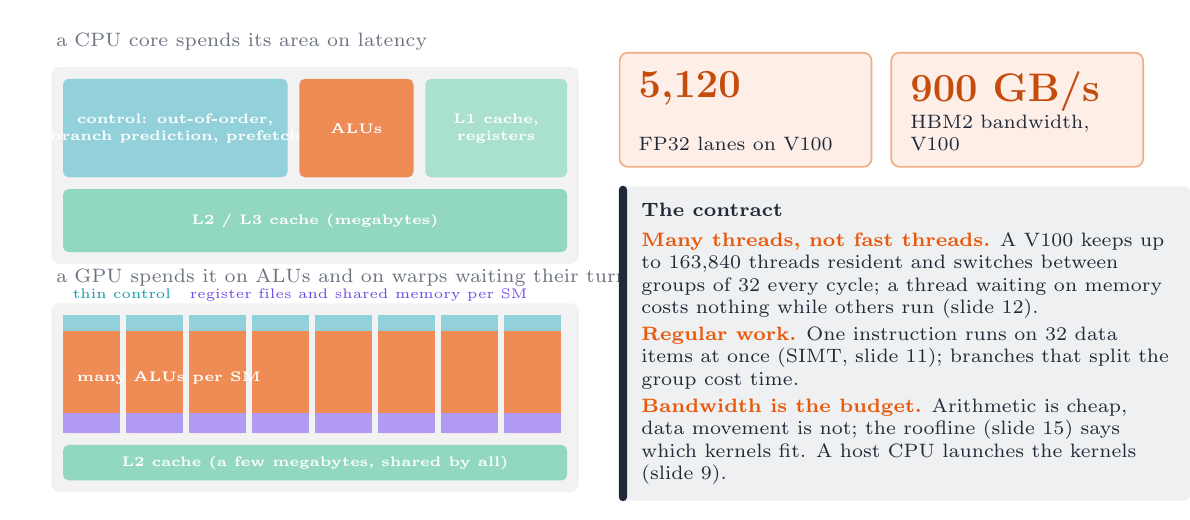
\begin{tikzpicture}
  \useasboundingbox (0,0) rectangle (14.4,5.9);
  % CPU cartoon
  \node[lab,anchor=south west] at (0.3,5.55) {a CPU core spends its area on latency};
  \begin{scope}[shift={(0.3,2.9)}]
    \fill[ink!6,rounded corners=3pt] (0,0) rectangle (6.7,2.5);
    \fill[emb!45,rounded corners=2pt] (0.15,0.15) rectangle (6.55,0.95);
    \node[font=\tiny\bfseries,text=white] at (3.35,0.55) {L2 / L3 cache (megabytes)};
    \fill[vc!45,rounded corners=2pt] (0.15,1.1) rectangle (3.0,2.35);
    \node[font=\tiny\bfseries,text=white,align=center] at (1.575,1.72) {control: out-of-order,\\branch prediction, prefetch};
    \fill[attn!70,rounded corners=2pt] (3.15,1.1) rectangle (4.6,2.35);
    \node[font=\tiny\bfseries,text=white,align=center] at (3.875,1.72) {ALUs};
    \fill[emb!35,rounded corners=2pt] (4.75,1.1) rectangle (6.55,2.35);
    \node[font=\tiny\bfseries,text=white,align=center] at (5.65,1.72) {L1 cache,\\registers};
  \end{scope}
  \node[lab,anchor=south west] at (0.3,2.55) {a GPU spends it on ALUs and on warps waiting their turn};
  \begin{scope}[shift={(0.3,0.0)}]
    \fill[ink!6,rounded corners=3pt] (0,0) rectangle (6.7,2.4);
    \fill[emb!45,rounded corners=2pt] (0.15,0.15) rectangle (6.55,0.6);
    \node[font=\tiny\bfseries,text=white] at (3.35,0.375) {L2 cache (a few megabytes, shared by all)};
    \foreach \c in {0,...,7}{
      \fill[attn!70,rounded corners=1.5pt] (0.15+\c*0.8,0.75) rectangle ++(0.72,1.5);
      \fill[vc!45] (0.15+\c*0.8,2.05) rectangle ++(0.72,0.2);
      \fill[posc!55] (0.15+\c*0.8,0.75) rectangle ++(0.72,0.25);}
    \node[font=\tiny,text=white,anchor=west] at (0.2,1.45) {\bfseries many ALUs per SM};
    \node[font=\tiny,text=muted,anchor=south west] at (0.15,2.3) {\textcolor{vc}{thin control}\quad \textcolor{posc}{register files and shared memory per SM}};
  \end{scope}
  \stat{7.5}{5.6}{5{,}120}{FP32 lanes on V100}{attn}
  \stat{10.95}{5.6}{900 GB/s}{HBM2 bandwidth, V100}{attn}
  \bgpanels{7.5}{3.9}{6.7cm}{The contract}{%
    \hl{attn}{Many threads, not fast threads.} A V100 keeps up to 163{,}840
    threads resident and switches between groups of 32 every cycle; a
    thread waiting on memory costs nothing while others run (slide 12).\\[2pt]
    \hl{attn}{Regular work.} One instruction runs on 32 data items at
    once (SIMT, slide 11); branches that split the group cost time.\\[2pt]
    \hl{attn}{Bandwidth is the budget.} Arithmetic is cheap, data
    movement is not; the roofline (slide 15) says which kernels fit.
    A host CPU launches the kernels (slide 9).}
\end{tikzpicture}
\end{frame}

% ---------------------------------------------------------------- 3
\begin{frame}{Three numbers: FLOP/s, bytes per second, watts}
\framesubtitle{Peak arithmetic grew about 45$\times$ from G80 to V100 while board power doubled; memory bandwidth grew about 10$\times$.}
\centering
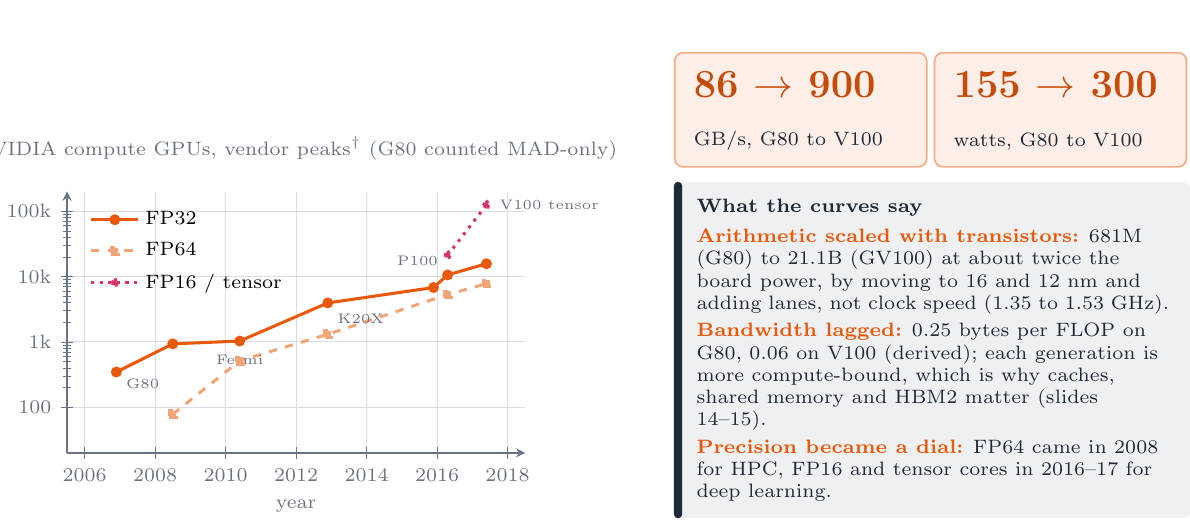
\begin{tikzpicture}
  \useasboundingbox (0,0) rectangle (14.4,5.9);
  \begin{scope}[shift={(0.5,0.5)}]
  \begin{axis}[lecture,width=7.4cm,height=4.9cm,ymode=log,xmin=2005.5,xmax=2018.5,ymin=20,ymax=200000,
      xlabel={year},ylabel={peak GFLOP/s (log scale)},
      xtick={2006,2008,2010,2012,2014,2016,2018},xticklabel style={/pgf/number format/1000 sep={}},scaled x ticks=false,
      ytick={100,1000,10000,100000},yticklabels={100,1k,10k,100k},
      legend pos=north west,legend style={at={(0.03,0.97)},anchor=north west},
      title style={font=\scriptsize,text=muted,at={(0.5,1.02)}},title={NVIDIA compute GPUs, vendor peaks$^\dagger$ (G80 counted MAD-only)}]
    \addplot[attn,line width=1.1pt,mark=*,mark size=1.4pt] coordinates {(2006.9,346) (2008.5,933) (2010.4,1030) (2012.9,3950) (2015.9,6800) (2016.3,10600) (2017.4,15700)};
    \addlegendentry{FP32}
    \addplot[attn!55,line width=1.1pt,dashed,mark=square*,mark size=1.2pt] coordinates {(2008.5,78) (2010.4,515) (2012.9,1310) (2016.3,5300) (2017.4,7800)};
    \addlegendentry{FP64}
    \addplot[outc,line width=1.1pt,dotted,mark=triangle*,mark size=1.6pt] coordinates {(2016.3,21200) (2017.4,125000)};
    \addlegendentry{FP16 / tensor}
    \node[font=\tiny,text=muted,anchor=west] at (axis cs:2006.9,230) {G80};
    \node[font=\tiny,text=muted,anchor=north] at (axis cs:2010.4,900) {Fermi};
    \node[font=\tiny,text=muted,anchor=north west] at (axis cs:2012.9,3700) {K20X};
    \node[font=\tiny,text=muted,anchor=south east] at (axis cs:2016.3,10600) {P100};
    \node[font=\tiny,text=muted,anchor=west] at (axis cs:2017.5,125000) {V100 tensor};
  \end{axis}
  \end{scope}
  \stat{8.2}{5.6}{86 $\to$ 900}{GB/s, G80 to V100}{attn}
  \stat{11.5}{5.6}{155 $\to$ 300}{watts, G80 to V100}{attn}
  \bgpanels{8.2}{3.95}{6.0cm}{What the curves say}{%
    \hl{attn}{Arithmetic scaled with transistors:} 681M (G80) to 21.1B
    (GV100) at about twice the board power, by moving to 16 and 12 nm
    and adding lanes, not clock speed (1.35 to 1.53 GHz).\\[2pt]
    \hl{attn}{Bandwidth lagged:} 0.25 bytes per FLOP on G80, 0.06 on
    V100 (derived); each generation is more compute-bound, which is why
    caches, shared memory and HBM2 matter (slides 14--15).\\[2pt]
    \hl{attn}{Precision became a dial:} FP64 came in 2008 for HPC,
    FP16 and tensor cores in 2016--17 for deep learning.}
\end{tikzpicture}
\end{frame}

% ---------------------------------------------------------------- 4
\begin{frame}{A timeline: from the Geometry Engine to Volta}
\framesubtitle{Thirty-five years in four moves: fixed function, programmable shaders, unified compute, specialized compute.}
\centering
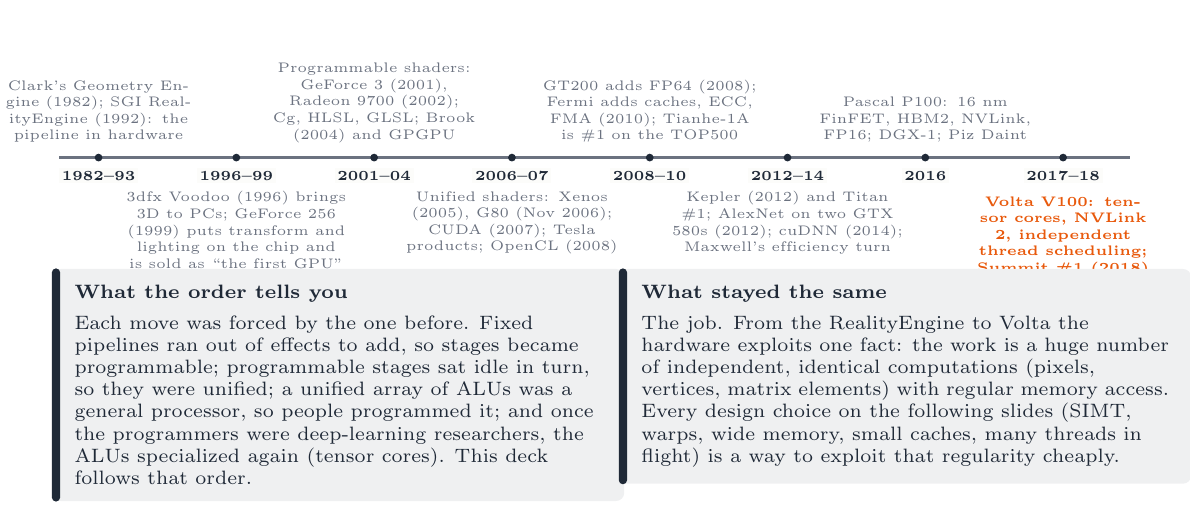
\begin{tikzpicture}
  \useasboundingbox (0,0) rectangle (14.4,5.9);
  \draw[muted,line width=0.8pt] (0.4,4.25) -- (14.0,4.25);
  \foreach \x in {0.9,2.65,4.4,6.15,7.9,9.65,11.4,13.15}{\fill[ink] (\x,4.25) circle (1.4pt);}
  \foreach \yr/\x in {1982--93/0.9,1996--99/2.65,2001--04/4.4,2006--07/6.15,2008--10/7.9,2012--14/9.65,2016/11.4,2017--18/13.15}{
    \node[font=\tiny\bfseries,text=ink,fill=paper,inner sep=1pt] at (\x,4.02) {\yr};}
  \node[lab,anchor=south,text width=3.0cm,align=center,font=\tiny] at (0.9,4.38) {Clark's Geometry Engine (1982); SGI RealityEngine (1992): the pipeline in hardware};
  \node[lab,anchor=north,text width=3.0cm,align=center,font=\tiny] at (2.65,3.88) {3dfx Voodoo (1996) brings 3D to PCs; GeForce 256 (1999) puts transform and lighting on the chip and is sold as ``the first GPU''};
  \node[lab,anchor=south,text width=3.0cm,align=center,font=\tiny] at (4.4,4.38) {Programmable shaders: GeForce 3 (2001), Radeon 9700 (2002); Cg, HLSL, GLSL; Brook (2004) and GPGPU};
  \node[lab,anchor=north,text width=3.0cm,align=center,font=\tiny] at (6.15,3.88) {Unified shaders: Xenos (2005), G80 (Nov 2006); CUDA (2007); Tesla products; OpenCL (2008)};
  \node[lab,anchor=south,text width=3.0cm,align=center,font=\tiny] at (7.9,4.38) {GT200 adds FP64 (2008); Fermi adds caches, ECC, FMA (2010); Tianhe-1A is \#1 on the TOP500};
  \node[lab,anchor=north,text width=3.0cm,align=center,font=\tiny] at (9.65,3.88) {Kepler (2012) and Titan \#1; AlexNet on two GTX 580s (2012); cuDNN (2014); Maxwell's efficiency turn};
  \node[lab,anchor=south,text width=3.0cm,align=center,font=\tiny] at (11.4,4.38) {Pascal P100: 16 nm FinFET, HBM2, NVLink, FP16; DGX-1; Piz Daint};
  \node[anchor=north,text width=2.8cm,align=center,font=\tiny\bfseries,text=attn] at (13.15,3.88) {Volta V100: tensor cores, NVLink 2, independent thread scheduling; Summit \#1 (2018)};
  \bgpanels{0.3}{2.85}{6.7cm}{What the order tells you}{%
    Each move was forced by the one before. Fixed pipelines ran out of
    effects to add, so stages became programmable; programmable stages
    sat idle in turn, so they were unified; a unified array of ALUs was
    a general processor, so people programmed it; and once the
    programmers were deep-learning researchers, the ALUs specialized
    again (tensor cores). This deck follows that order.}
  \bgpanels{7.5}{2.85}{6.7cm}{What stayed the same}{%
    The job. From the RealityEngine to Volta the hardware exploits one
    fact: the work is a huge number of independent, identical
    computations (pixels, vertices, matrix elements) with regular memory
    access. Every design choice on the following slides (SIMT, warps,
    wide memory, small caches, many threads in flight) is a way to
    exploit that regularity cheaply.}
\end{tikzpicture}
\end{frame}

% ---------------------------------------------------------------- 5
\stage{2}
\begin{frame}{The fixed-function graphics pipeline}
\framesubtitle{Vertices in, pixels out: a hardware assembly line whose stages were fixed in silicon until 2001.}
\centering
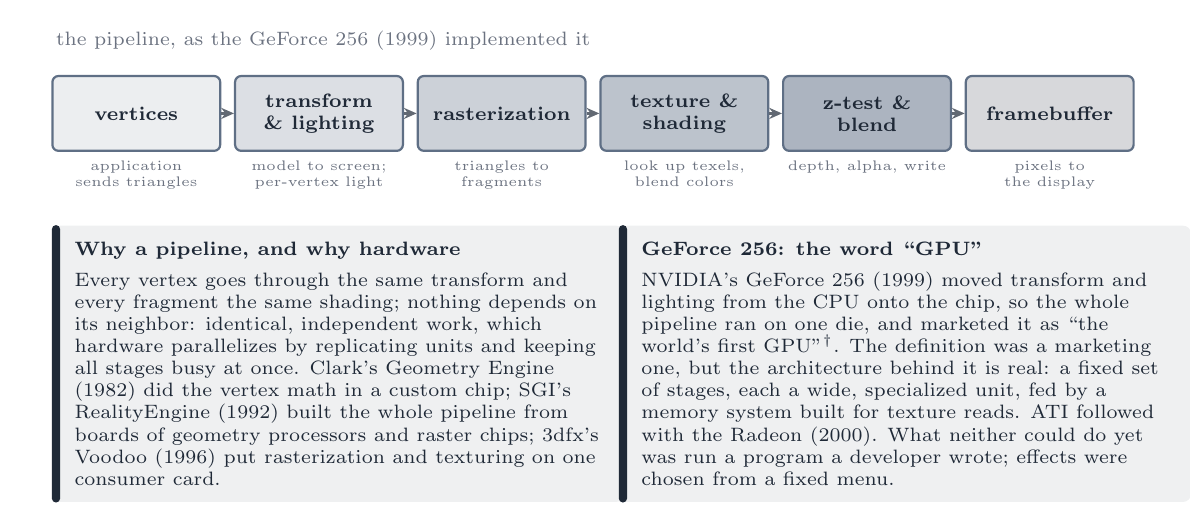
\begin{tikzpicture}
  \useasboundingbox (0,0) rectangle (14.4,5.9);
  \node[lab,anchor=south west] at (0.3,5.55) {the pipeline, as the GeForce 256 (1999) implemented it};
  \foreach \i/\name/\sub/\c in {0/vertices/{application sends triangles}/tok!12, 1/transform \& lighting/{model to screen; per-vertex light}/tok!22, 2/rasterization/{triangles to fragments}/tok!32, 3/texture \& shading/{look up texels{,} blend colors}/tok!42, 4/z-test \& blend/{depth{,} alpha{,} write}/tok!52, 5/framebuffer/{pixels to the display}/ink!18}{
    \node[comp=tok,fill=\c,text width=1.85cm,minimum height=0.95cm,font=\scriptsize\bfseries,text=ink,align=center,anchor=north west] (s\i) at (0.3+\i*2.32,5.3) {\name};
    \node[lab,font=\tiny,anchor=north,text width=2.1cm,align=center] at ($(s\i.south)+(0,-0.05)$) {\sub};}
  \foreach \i [evaluate=\i as \j using int(\i+1)] in {0,...,4}{\draw[flow] (s\i.east) -- (s\j.west);}
  \bgpanels{0.3}{3.4}{6.7cm}{Why a pipeline, and why hardware}{%
    Every vertex goes through the same transform and every fragment
    the same shading; nothing depends on its neighbor: identical,
    independent work, which hardware parallelizes by replicating units
    and keeping all stages busy at once. Clark's Geometry Engine (1982)
    did the vertex math in a custom chip; SGI's RealityEngine (1992)
    built the whole pipeline from boards of geometry processors and
    raster chips; 3dfx's Voodoo (1996) put rasterization and texturing
    on one consumer card.}
  \bgpanels{7.5}{3.4}{6.7cm}{GeForce 256: the word ``GPU''}{%
    NVIDIA's GeForce 256 (1999) moved transform and lighting from the
    CPU onto the chip, so the whole pipeline ran on one die, and
    marketed it as ``the world's first GPU''$^\dagger$. The definition
    was a marketing one, but the architecture behind it is real: a
    fixed set of stages, each a wide, specialized unit, fed by a
    memory system built for texture reads. ATI followed with the Radeon
    (2000). What neither could do yet was run a program a developer
    wrote; effects were chosen from a fixed menu.}
\end{tikzpicture}
\end{frame}

% ---------------------------------------------------------------- 6
\begin{frame}{Programmable shaders: a processor hiding in each stage}
\framesubtitle{2001--2004: vertex and pixel stages become small SIMD processors; separate units per stage leave silicon idle.}
\centering
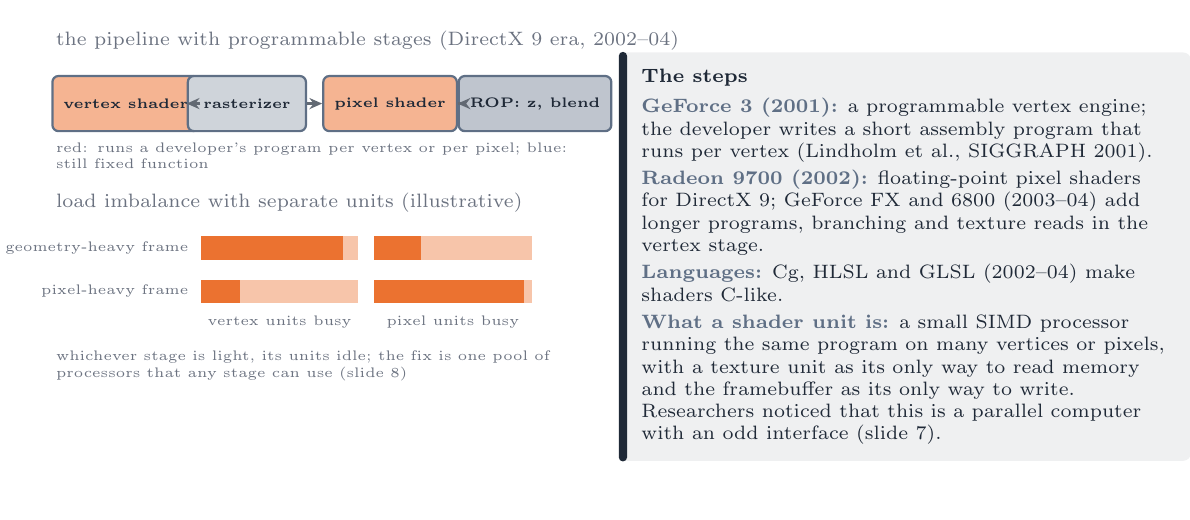
\begin{tikzpicture}
  \useasboundingbox (0,0) rectangle (14.4,5.9);
  \node[lab,anchor=south west] at (0.3,5.55) {the pipeline with programmable stages (DirectX 9 era, 2002--04)};
  \foreach \i/\name/\c in {0/vertex shader/attn!45, 1/rasterizer/tok!30, 2/pixel shader/attn!45, 3/ROP: z{,} blend/tok!40}{
    \node[comp=tok,fill=\c,minimum width=1.5cm,minimum height=0.7cm,font=\tiny\bfseries,text=ink,anchor=north west] (p\i) at (0.3+\i*1.72,5.3) {\name};}
  \foreach \i [evaluate=\i as \j using int(\i+1)] in {0,...,2}{\draw[flow] (p\i.east) -- (p\j.west);}
  \node[lab,font=\tiny,anchor=north west,text width=6.7cm] at (0.3,4.5) {red: runs a developer's program per vertex or per pixel; blue: still fixed function};
  % load imbalance bars
  \node[lab,anchor=south west] at (0.3,3.5) {load imbalance with separate units (illustrative)};
  \foreach \k/\y/\v/\p/\lbl in {0/2.95/0.9/0.3/{geometry-heavy frame}, 1/2.4/0.25/0.95/{pixel-heavy frame}}{
    \node[lab,font=\tiny,anchor=east] at (2.1,\y+0.15) {\lbl};
    \fill[attn!35] (2.2,\y) rectangle ++(2.0,0.3); \fill[attn!85] (2.2,\y) rectangle ++(2.0*\v,0.3);
    \fill[attn!35] (4.4,\y) rectangle ++(2.0,0.3); \fill[attn!85] (4.4,\y) rectangle ++(2.0*\p,0.3);}
  \node[lab,font=\tiny,anchor=north] at (3.2,2.3) {vertex units busy};
  \node[lab,font=\tiny,anchor=north] at (5.4,2.3) {pixel units busy};
  \node[lab,font=\tiny,anchor=north west,text width=6.7cm] at (0.3,1.85) {whichever stage is light, its units idle; the fix is one pool of processors that any stage can use (slide 8)};
  \bgpanels{7.5}{5.6}{6.7cm}{The steps}{%
    \hl{tok}{GeForce 3 (2001):} a programmable vertex engine; the
    developer writes a short assembly program that runs per vertex
    (Lindholm et al., SIGGRAPH 2001).\\[2pt]
    \hl{tok}{Radeon 9700 (2002):} floating-point pixel shaders for
    DirectX 9; GeForce FX and 6800 (2003--04) add longer programs,
    branching and texture reads in the vertex stage.\\[2pt]
    \hl{tok}{Languages:} Cg, HLSL and GLSL (2002--04) make shaders C-like.\\[2pt]
    \hl{tok}{What a shader unit is:} a small SIMD processor running the
    same program on many vertices or pixels, with a texture unit as its
    only way to read memory and the framebuffer as its only way to
    write. Researchers noticed that this is a parallel computer with an
    odd interface (slide 7).}
\end{tikzpicture}
\end{frame}

% ---------------------------------------------------------------- 7
\stage{3}
\begin{frame}{GPGPU: computing with pixels}
\framesubtitle{2003--2006: arrays became textures, kernels became fragment shaders, and a graphics API hid a parallel computer.}
\centering
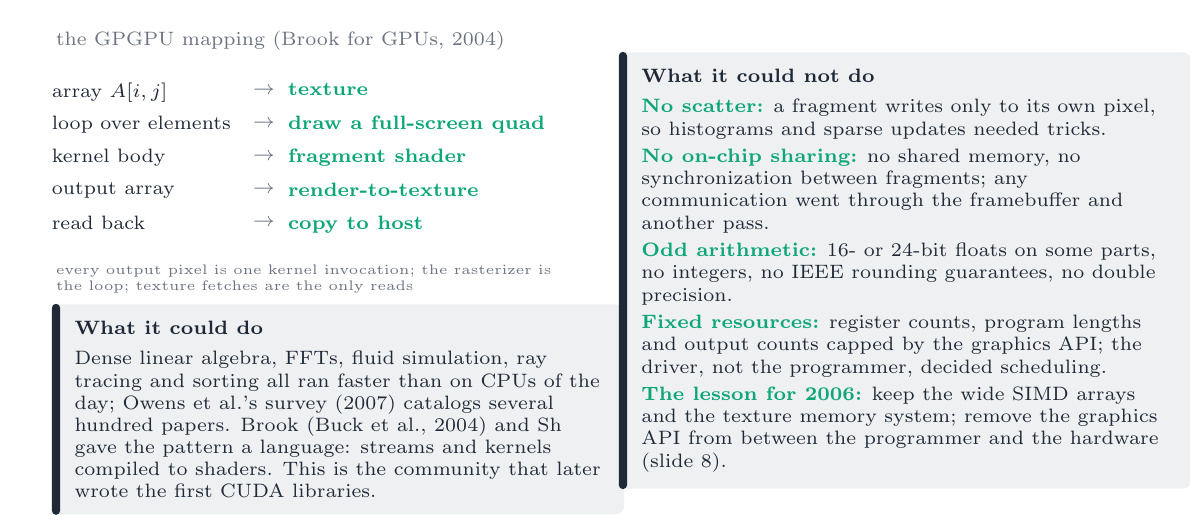
\begin{tikzpicture}
  \useasboundingbox (0,0) rectangle (14.4,5.9);
  \node[lab,anchor=south west] at (0.3,5.55) {the GPGPU mapping (Brook for GPUs, 2004)};
  \foreach \i/\a/\b in {0/{array $A[i,j]$}/{texture}, 1/{loop over elements}/{draw a full-screen quad}, 2/{kernel body}/{fragment shader}, 3/{output array}/{render-to-texture}, 4/{read back}/{copy to host}}{
    \node[anchor=north west,font=\scriptsize,text=ink,inner sep=0] at (0.3,5.2-\i*0.42) {\a};
    \node[font=\scriptsize,text=muted] at (3.0,5.1-\i*0.42) {$\to$};
    \node[anchor=north west,font=\scriptsize\bfseries,text=emb,inner sep=0] at (3.3,5.2-\i*0.42) {\b};}
  \node[lab,font=\tiny,anchor=north west,text width=6.7cm] at (0.3,2.95) {every output pixel is one kernel invocation; the rasterizer is the loop; texture fetches are the only reads};
  \bgpanels{0.3}{2.4}{6.7cm}{What it could do}{%
    Dense linear algebra, FFTs, fluid simulation, ray tracing and
    sorting all ran faster than on CPUs of the day; Owens et al.'s survey
    (2007) catalogs several hundred papers. Brook (Buck et al., 2004)
    and Sh gave the pattern a language: streams and kernels compiled to
    shaders. This is the community that later wrote the first CUDA
    libraries.}
  \bgpanels{7.5}{5.6}{6.7cm}{What it could not do}{%
    \hl{emb}{No scatter:} a fragment writes only to its own pixel, so
    histograms and sparse updates needed tricks.\\[2pt]
    \hl{emb}{No on-chip sharing:} no shared memory, no synchronization
    between fragments; any communication went through the framebuffer
    and another pass.\\[2pt]
    \hl{emb}{Odd arithmetic:} 16- or 24-bit floats on some parts, no
    integers, no IEEE rounding guarantees, no double precision.\\[2pt]
    \hl{emb}{Fixed resources:} register counts, program lengths and
    output counts capped by the graphics API; the driver, not the
    programmer, decided scheduling.\\[2pt]
    \hl{emb}{The lesson for 2006:} keep the wide SIMD arrays and the
    texture memory system; remove the graphics API from between the
    programmer and the hardware (slide 8).}
\end{tikzpicture}
\end{frame}

% ---------------------------------------------------------------- 8
\begin{frame}{G80 (2006): one unified array of processors, and CUDA}
\framesubtitle{The GeForce 8800 GTX replaced separate vertex and pixel units with 128 identical processors, then got a C compiler.}
\centering
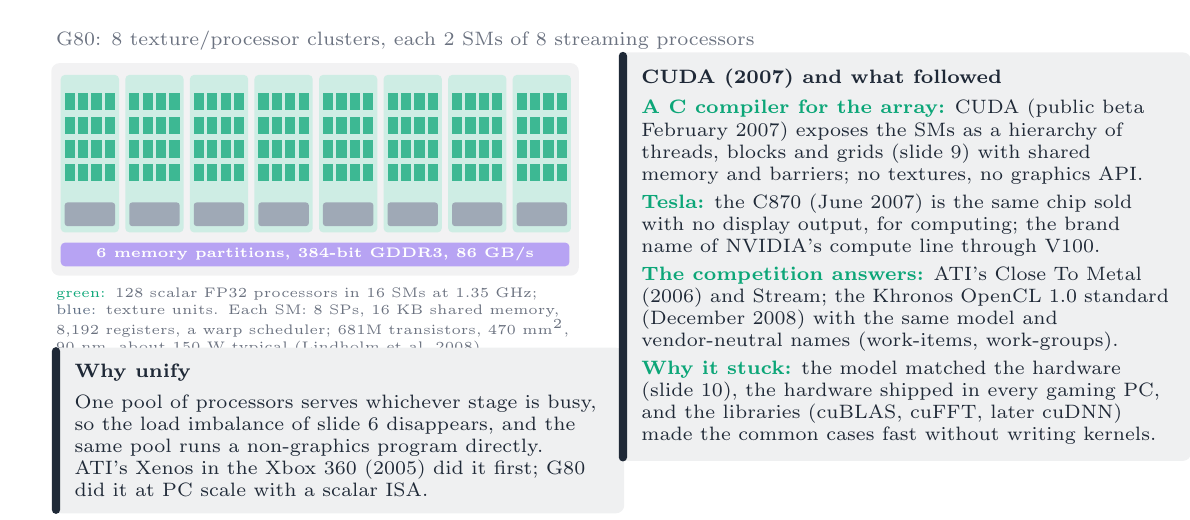
\begin{tikzpicture}
  \useasboundingbox (0,0) rectangle (14.4,5.9);
  \node[lab,anchor=south west] at (0.3,5.55) {G80: 8 texture/processor clusters, each 2 SMs of 8 streaming processors};
  \begin{scope}[shift={(0.3,2.75)}]
    \fill[ink!6,rounded corners=3pt] (0,0) rectangle (6.7,2.7);
    \foreach \c in {0,...,7}{
      \begin{scope}[shift={(0.12+\c*0.82,0.55)}]
        \fill[emb!20,rounded corners=1.5pt] (0,0) rectangle (0.74,2.0);
        \foreach \r in {0,...,3}{\foreach \k in {0,...,3}{
          \fill[emb!80] (0.05+\k*0.17,1.55-\r*0.3) rectangle ++(0.13,0.22);}}
        \fill[tok!60,rounded corners=1pt] (0.05,0.08) rectangle (0.69,0.38);
      \end{scope}}
    \node[font=\tiny,text=muted,anchor=south west] at (0.1,2.08) {};
    \fill[posc!50,rounded corners=1.5pt] (0.12,0.12) rectangle (6.58,0.42);
    \node[font=\tiny\bfseries,text=white] at (3.35,0.27) {6 memory partitions, 384-bit GDDR3, 86 GB/s};
  \end{scope}
  \node[lab,font=\tiny,anchor=north west,text width=6.7cm] at (0.3,2.65) {\textcolor{emb}{green:} 128 scalar FP32 processors in 16 SMs at 1.35 GHz; \textcolor{tok}{blue:} texture units. Each SM: 8 SPs, 16 KB shared memory, 8{,}192 registers, a warp scheduler; 681M transistors, 470 mm$^2$, 90 nm, about 150 W typical (Lindholm et al.\ 2008)};
  \bgpanels{0.3}{1.85}{6.7cm}{Why unify}{%
    One pool of processors serves whichever stage is busy, so the load
    imbalance of slide 6 disappears, and the same pool runs a
    non-graphics program directly. ATI's Xenos in the Xbox 360 (2005)
    did it first; G80 did it at PC scale with a scalar ISA.}
  \bgpanels{7.5}{5.6}{6.7cm}{CUDA (2007) and what followed}{%
    \hl{emb}{A C compiler for the array:} CUDA (public beta February
    2007) exposes the SMs as a hierarchy of threads, blocks and grids
    (slide 9) with shared memory and barriers; no textures, no
    graphics API.\\[2pt]
    \hl{emb}{Tesla:} the C870 (June 2007) is the same chip sold with no
    display output, for computing; the brand name of NVIDIA's compute
    line through V100.\\[2pt]
    \hl{emb}{The competition answers:} ATI's Close To Metal (2006) and
    Stream; the Khronos OpenCL 1.0 standard (December 2008) with the
    same model and vendor-neutral names (work-items, work-groups).\\[2pt]
    \hl{emb}{Why it stuck:} the model matched the hardware (slide 10),
    the hardware shipped in every gaming PC, and the libraries
    (cuBLAS, cuFFT, later cuDNN) made the common cases fast without
    writing kernels.}
\end{tikzpicture}
\end{frame}

% ---------------------------------------------------------------- 9
\stage{4}
\begin{frame}{The CUDA programming model: grids of blocks of threads}
\framesubtitle{Write the program for one thread; launch tens of thousands; let the hardware schedule blocks onto SMs.}
\centering
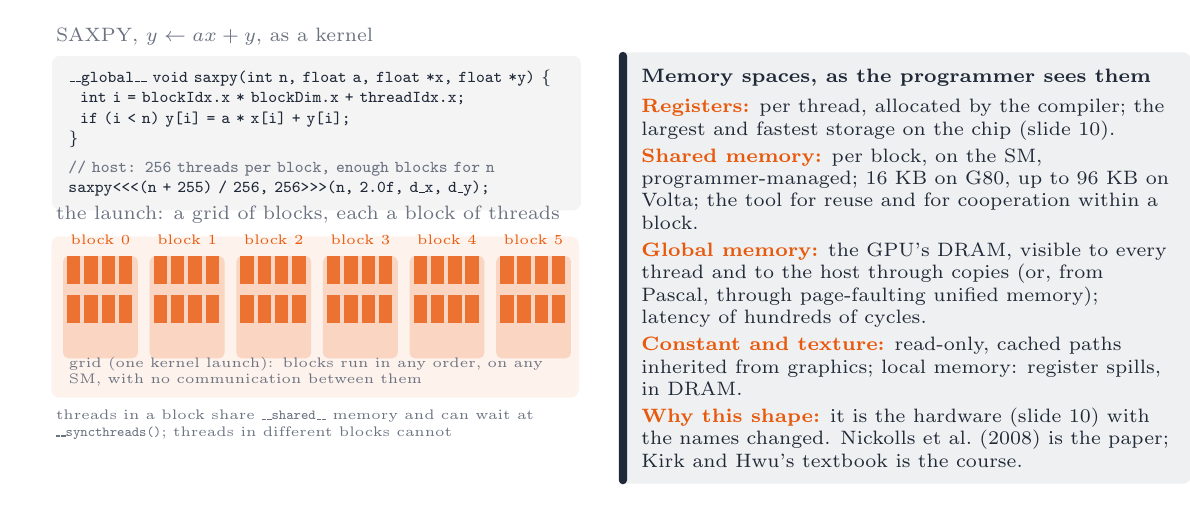
\begin{tikzpicture}
  \useasboundingbox (0,0) rectangle (14.4,5.9);
  \node[lab,anchor=south west] at (0.3,5.62) {SAXPY, $y \leftarrow a x + y$, as a kernel};
  \node[anchor=north west,inner sep=0,font=\ttfamily\fontsize{6.2}{7.4}\selectfont,text=ink,
        rounded corners=3pt,fill=ink!5,inner xsep=6pt,inner ysep=5pt,text width=6.3cm,align=left] at (0.3,5.55) {%
    \_\_global\_\_ void saxpy(int n, float a, float *x, float *y) \{\\
    \ \ int i = blockIdx.x * blockDim.x + threadIdx.x;\\
    \ \ if (i < n) y[i] = a * x[i] + y[i];\\
    \}\\[3pt]
    {\color{muted}// host: 256 threads per block, enough blocks for n}\\
    saxpy<<<(n + 255) / 256, 256>>>(n, 2.0f, d\_x, d\_y);};
  % grid diagram
  \node[lab,anchor=south west] at (0.3,3.35) {the launch: a grid of blocks, each a block of threads};
  \begin{scope}[shift={(0.3,1.2)}]
    \fill[attn!8,rounded corners=3pt] (0,0) rectangle (6.7,2.05);
    \foreach \b in {0,...,5}{
      \fill[attn!25,rounded corners=2pt] (0.15+\b*1.1,0.5) rectangle ++(0.95,1.3);
      \foreach \t in {0,...,7}{\fill[attn!85] ({0.2+\b*1.1+mod(\t,4)*0.22},{1.45-floor(\t/4)*0.5}) rectangle ++(0.17,0.35);}
      \node[font=\tiny,text=attn,anchor=south] at (0.625+\b*1.1,1.82) {block \b};}
    \node[font=\tiny,text=muted,anchor=south west,text width=6.5cm] at (0.1,0.02) {grid (one kernel launch): blocks run in any order, on any SM, with no communication between them};
  \end{scope}
  \node[lab,font=\tiny,anchor=north west,text width=6.7cm] at (0.3,1.1) {threads in a block share \texttt{\_\_shared\_\_} memory and can wait at \texttt{\_\_syncthreads()}; threads in different blocks cannot};
  \bgpanels{7.5}{5.6}{6.7cm}{Memory spaces, as the programmer sees them}{%
    \hl{attn}{Registers:} per thread, allocated by the compiler;
    the largest and fastest storage on the chip (slide 10).\\[2pt]
    \hl{attn}{Shared memory:} per block, on the SM, programmer-managed;
    16 KB on G80, up to 96 KB on Volta; the tool for reuse and for
    cooperation within a block.\\[2pt]
    \hl{attn}{Global memory:} the GPU's DRAM, visible to every thread
    and to the host through copies (or, from Pascal, through
    page-faulting unified memory); latency of hundreds of cycles.\\[2pt]
    \hl{attn}{Constant and texture:} read-only, cached paths inherited
    from graphics; local memory: register spills, in DRAM.\\[2pt]
    \hl{attn}{Why this shape:} it is the hardware (slide 10) with the
    names changed. Nickolls et al.\ (2008) is the paper; Kirk and Hwu's
    textbook is the course.}
\end{tikzpicture}
\end{frame}

% ---------------------------------------------------------------- 10
\begin{frame}{Mapping the model to the chip: blocks to SMs, threads to warps}
\framesubtitle{A streaming multiprocessor runs several blocks at once; its scheduler issues one instruction for 32 threads at a time.}
\centering
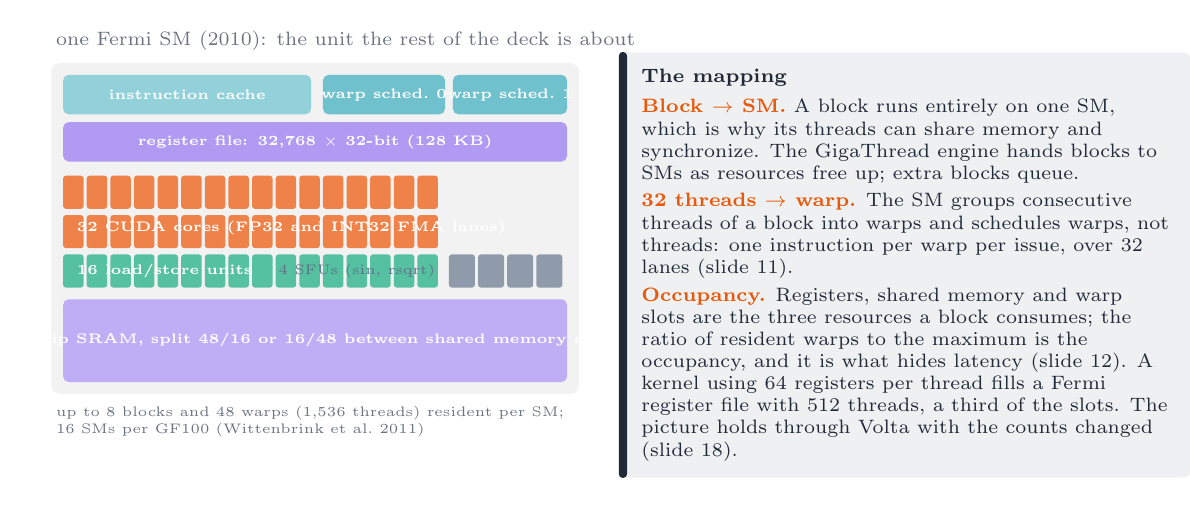
\begin{tikzpicture}
  \useasboundingbox (0,0) rectangle (14.4,5.9);
  \node[lab,anchor=south west] at (0.3,5.55) {one Fermi SM (2010): the unit the rest of the deck is about};
  \begin{scope}[shift={(0.3,1.25)}]
    \fill[ink!6,rounded corners=3pt] (0,0) rectangle (6.7,4.2);
    \fill[vc!45,rounded corners=2pt] (0.15,3.55) rectangle (3.3,4.05);
    \node[font=\tiny\bfseries,text=white] at (1.725,3.8) {instruction cache};
    \fill[vc!60,rounded corners=2pt] (3.45,3.55) rectangle (5.0,4.05);
    \node[font=\tiny\bfseries,text=white,align=center] at (4.225,3.8) {warp sched.\ 0};
    \fill[vc!60,rounded corners=2pt] (5.1,3.55) rectangle (6.55,4.05);
    \node[font=\tiny\bfseries,text=white,align=center] at (5.825,3.8) {warp sched.\ 1};
    \fill[posc!55,rounded corners=2pt] (0.15,2.95) rectangle (6.55,3.45);
    \node[font=\tiny\bfseries,text=white] at (3.35,3.2) {register file: 32{,}768 $\times$ 32-bit (128 KB)};
    \foreach \r in {0,1}{\foreach \c in {0,...,15}{\fill[attn!75,rounded corners=1pt] (0.15+\c*0.3,2.35-\r*0.5) rectangle ++(0.26,0.42);}}
    \node[font=\tiny\bfseries,text=white,anchor=west] at (0.2,2.1) {32 CUDA cores (FP32 and INT32 FMA lanes)};
    \foreach \c in {0,...,15}{\fill[emb!70,rounded corners=1pt] (0.15+\c*0.3,1.35) rectangle ++(0.26,0.42);}
    \node[font=\tiny\bfseries,text=white,anchor=west] at (0.2,1.56) {16 load/store units};
    \foreach \c in {0,...,3}{\fill[tok!70,rounded corners=1pt] (5.05+\c*0.37,1.35) rectangle ++(0.33,0.42);}
    \node[font=\tiny,text=tok,anchor=east] at (5.0,1.56) {4 SFUs (sin, rsqrt)};
    \fill[posc!45,rounded corners=2pt] (0.15,0.15) rectangle (6.55,1.2);
    \node[font=\tiny\bfseries,text=white,align=center] at (3.35,0.68) {64 KB on-chip SRAM, split 48/16 or 16/48 between shared memory and L1 cache};
  \end{scope}
  \node[lab,font=\tiny,anchor=north west,text width=6.7cm] at (0.3,1.15) {up to 8 blocks and 48 warps (1{,}536 threads) resident per SM; 16 SMs per GF100 (Wittenbrink et al.\ 2011)};
  \bgpanels{7.5}{5.6}{6.7cm}{The mapping}{%
    \hl{attn}{Block $\to$ SM.} A block runs entirely on one SM, which is
    why its threads can share memory and synchronize. The GigaThread
    engine hands blocks to SMs as resources free up; extra blocks
    queue.\\[2pt]
    \hl{attn}{32 threads $\to$ warp.} The SM groups consecutive threads
    of a block into warps and schedules warps, not threads: one
    instruction per warp per issue, over 32 lanes (slide 11).\\[2pt]
    \hl{attn}{Occupancy.} Registers, shared memory and warp slots are
    the three resources a block consumes; the ratio of resident warps to
    the maximum is the occupancy, and it is what hides latency (slide
    12). A kernel using 64 registers per thread fills a Fermi register
    file with 512 threads, a third of the slots. The picture holds
    through Volta with the counts changed (slide 18).}
\end{tikzpicture}
\end{frame}

% ---------------------------------------------------------------- 11
\stage{5}
\begin{frame}{SIMT: SIMD hardware with a thread's face}
\framesubtitle{One instruction, 32 lanes, each lane its own thread: branches are allowed and divergent branches are paid for in time.}
\centering
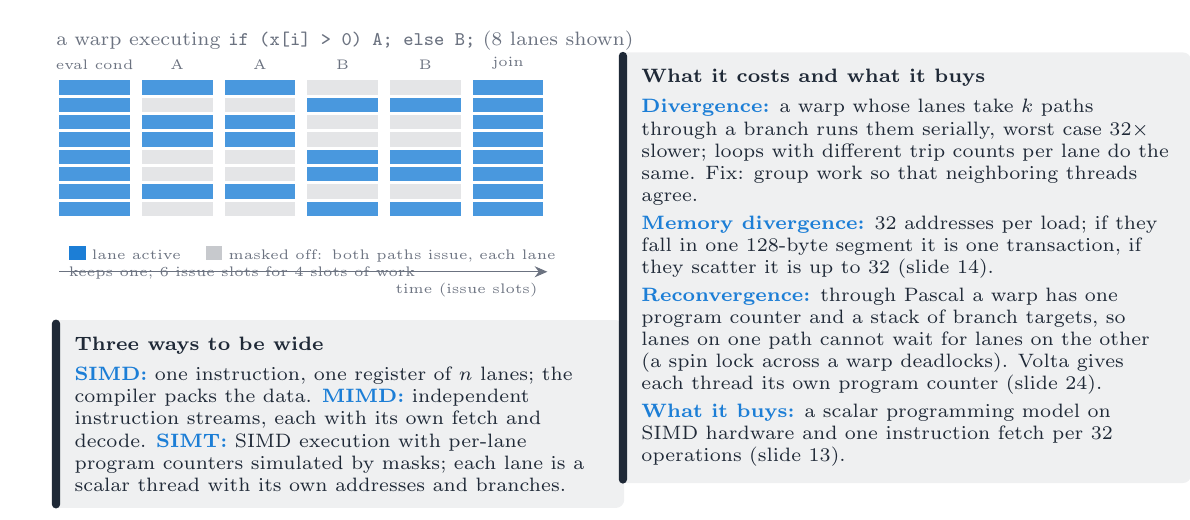
\begin{tikzpicture}
  \useasboundingbox (0,0) rectangle (14.4,5.9);
  \node[lab,anchor=south west] at (0.3,5.55) {a warp executing \texttt{if (x[i] > 0) A; else B;} (8 lanes shown)};
  \begin{scope}[shift={(0.3,3.3)}]
    \foreach \t/\lbl in {0/{eval cond},1/{A},2/{A},3/{B},4/{B},5/{join}}{
      \node[font=\tiny,text=muted,anchor=south] at (0.55+\t*1.05,1.95) {\lbl};}
    \foreach \l in {0,...,7}{
      \pgfmathsetmacro{\act}{(\l==0||\l==2||\l==3||\l==6)?1:0}
      \fill[mlp!80] (0.1,1.75-\l*0.22) rectangle ++(0.9,0.18);
      \ifnum\act=1
        \fill[mlp!80] (1.15,1.75-\l*0.22) rectangle ++(0.9,0.18); \fill[mlp!80] (2.2,1.75-\l*0.22) rectangle ++(0.9,0.18);
        \fill[ink!12] (3.25,1.75-\l*0.22) rectangle ++(0.9,0.18); \fill[ink!12] (4.3,1.75-\l*0.22) rectangle ++(0.9,0.18);
      \else
        \fill[ink!12] (1.15,1.75-\l*0.22) rectangle ++(0.9,0.18); \fill[ink!12] (2.2,1.75-\l*0.22) rectangle ++(0.9,0.18);
        \fill[mlp!80] (3.25,1.75-\l*0.22) rectangle ++(0.9,0.18); \fill[mlp!80] (4.3,1.75-\l*0.22) rectangle ++(0.9,0.18);
      \fi
      \fill[mlp!80] (5.35,1.75-\l*0.22) rectangle ++(0.9,0.18);}
    \node[font=\tiny,text=muted,anchor=north west,text width=6.5cm] at (0.1,-0.05) {\textcolor{mlp}{\rule{6pt}{5pt}} lane active \quad \textcolor{ink!25}{\rule{6pt}{5pt}} masked off: both paths issue, each lane keeps one; 6 issue slots for 4 slots of work};
    \draw[muted,line width=0.4pt,->] (0.1,-0.5) -- (6.3,-0.5); \node[font=\tiny,text=muted,anchor=north east] at (6.3,-0.52) {time (issue slots)};
  \end{scope}
  \bgpanels{0.3}{2.2}{6.7cm}{Three ways to be wide}{%
    \hl{mlp}{SIMD:} one instruction, one register of $n$ lanes; the
    compiler packs the data. \hl{mlp}{MIMD:} independent instruction
    streams, each with its own fetch and decode. \hl{mlp}{SIMT:} SIMD
    execution with per-lane program counters simulated by masks; each
    lane is a scalar thread with its own addresses and branches.}
  \bgpanels{7.5}{5.6}{6.7cm}{What it costs and what it buys}{%
    \hl{mlp}{Divergence:} a warp whose lanes take $k$ paths through a
    branch runs them serially, worst case 32$\times$ slower; loops with
    different trip counts per lane do the same. Fix: group work so that
    neighboring threads agree.\\[2pt]
    \hl{mlp}{Memory divergence:} 32 addresses per load; if they fall in
    one 128-byte segment it is one transaction, if they scatter it is
    up to 32 (slide 14).\\[2pt]
    \hl{mlp}{Reconvergence:} through Pascal a warp has one program
    counter and a stack of branch targets, so lanes on one path cannot
    wait for lanes on the other (a spin lock across a warp deadlocks).
    Volta gives each thread its own program counter (slide 24).\\[2pt]
    \hl{mlp}{What it buys:} a scalar programming model on SIMD hardware
    and one instruction fetch per 32 operations (slide 13).}
\end{tikzpicture}
\end{frame}

% ---------------------------------------------------------------- 12
\begin{frame}{Latency hiding: enough threads in flight to cover the memory}
\framesubtitle{A warp that waits on DRAM is parked and another issues; Little's law says how many must be in flight to keep DRAM busy.}
\centering
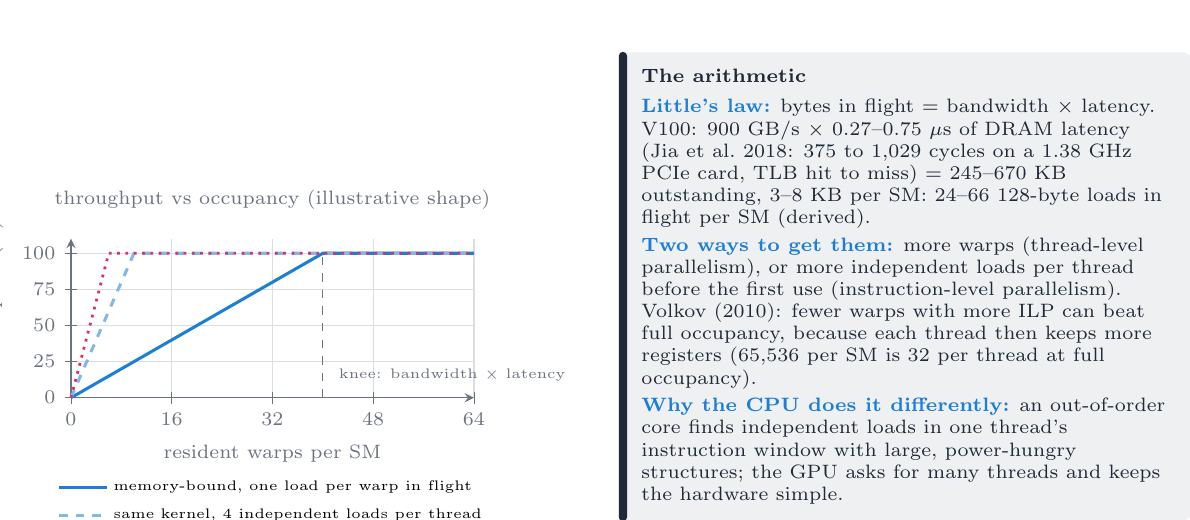
\begin{tikzpicture}
  \useasboundingbox (0,0) rectangle (14.4,5.9);
  \begin{scope}[shift={(0.55,1.2)}]
  \begin{axis}[lecture,width=6.7cm,height=3.6cm,xmin=0,xmax=64,ymin=0,ymax=110,
      xlabel={resident warps per SM},ylabel={fraction of peak (\%)},
      xtick={0,16,32,48,64},ytick={0,25,50,75,100},
      legend style={at={(0.5,-0.45)},anchor=north,legend columns=1,font=\tiny},
      title style={font=\scriptsize,text=muted,at={(0.5,1.02)}},title={throughput vs occupancy (illustrative shape)}]
    \addplot[mlp,line width=1.1pt,domain=0:64,samples=65] {100*min(1,x/40)};
    \addlegendentry{memory-bound, one load per warp in flight}
    \addplot[mlp!55,line width=1.1pt,dashed,domain=0:64,samples=65] {100*min(1,x/10)};
    \addlegendentry{same kernel, 4 independent loads per thread}
    \addplot[outc,line width=1.0pt,dotted,domain=0:64,samples=65] {100*min(1,x/6)};
    \addlegendentry{arithmetic-bound (short latencies)}
    \draw[muted,dashed] (axis cs:40,0) -- (axis cs:40,100);
    \node[font=\tiny,text=muted,anchor=south west] at (axis cs:41,5) {knee: bandwidth $\times$ latency};
  \end{axis}
  \end{scope}
  \bgpanels{7.5}{5.6}{6.7cm}{The arithmetic}{%
    \hl{mlp}{Little's law:} bytes in flight $=$ bandwidth $\times$
    latency. V100: 900 GB/s $\times$ 0.27--0.75 $\mu$s of DRAM latency
    (Jia et al.\ 2018: 375 to 1{,}029 cycles on a 1.38 GHz PCIe card,
    TLB hit to miss) $=$ 245--670 KB outstanding, 3--8 KB per SM: 24--66
    128-byte loads in flight per SM (derived).\\[2pt]
    \hl{mlp}{Two ways to get them:} more warps (thread-level
    parallelism), or more independent loads per thread before the first
    use (instruction-level parallelism). Volkov (2010): fewer warps with
    more ILP can beat full occupancy, because each thread then keeps
    more registers (65{,}536 per SM is 32 per thread at full
    occupancy).\\[2pt]
    \hl{mlp}{Why the CPU does it differently:} an out-of-order core
    finds independent loads in one thread's instruction window with
    large, power-hungry structures; the GPU asks for many threads and
    keeps the hardware simple.}
\end{tikzpicture}
\end{frame}

% ---------------------------------------------------------------- 13
\begin{frame}{Energy is the real constraint: why the design is what it is}
\framesubtitle{After Dennard scaling ended (about 2005), performance per watt decided the design; moving data costs more than math.}
\centering
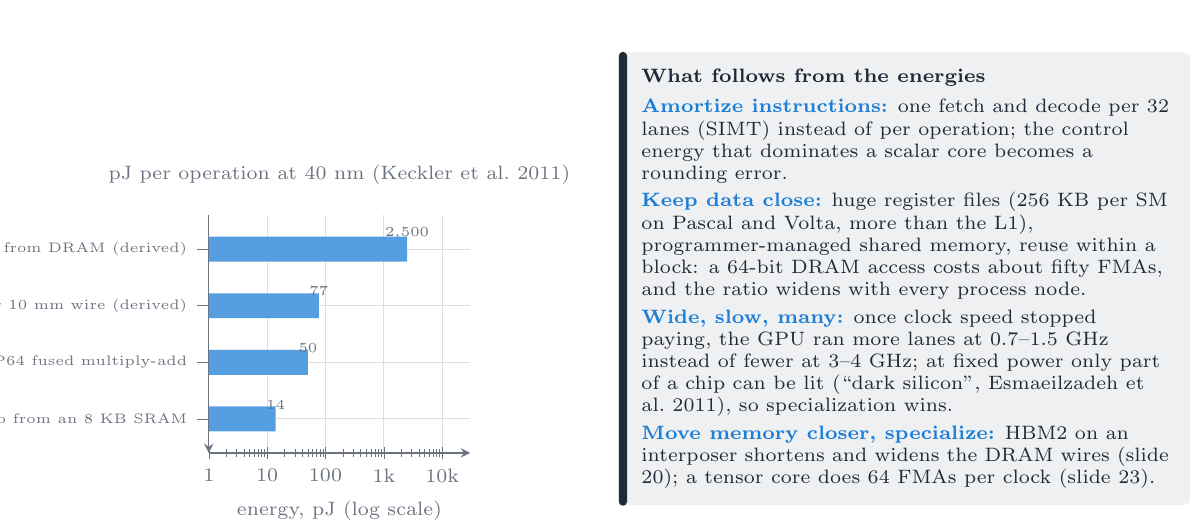
\begin{tikzpicture}
  \useasboundingbox (0,0) rectangle (14.4,5.9);
  \begin{scope}[shift={(2.3,0.5)}]
  \begin{axis}[lecture,width=4.9cm,height=4.6cm,xbar,xmode=log,xmin=1,xmax=30000,
      symbolic y coords={{64 b from DRAM (derived)},{64 b over 10 mm wire (derived)},{FP64 fused multiply-add},{64 b from an 8 KB SRAM}},
      ytick=data,y dir=reverse,yticklabel style={font=\tiny},xlabel={energy, pJ (log scale)},
      xtick={1,10,100,1000,10000},xticklabels={1,10,100,1k,10k},
      bar width=9pt,enlarge y limits=0.2,
      title style={font=\scriptsize,text=muted,at={(0.5,1.02)}},title={pJ per operation at 40 nm (Keckler et al.\ 2011)},
      nodes near coords,nodes near coords style={font=\tiny,text=muted},point meta=rawx]
    \addplot[fill=mlp!75,draw=none] coordinates {(2500,{64 b from DRAM (derived)}) (77,{64 b over 10 mm wire (derived)}) (50,{FP64 fused multiply-add}) (14,{64 b from an 8 KB SRAM})};
  \end{axis}
  \end{scope}
  \bgpanels{7.5}{5.6}{6.7cm}{What follows from the energies}{%
    \hl{mlp}{Amortize instructions:} one fetch and decode per 32 lanes
    (SIMT) instead of per operation; the control energy that dominates
    a scalar core becomes a rounding error.\\[2pt]
    \hl{mlp}{Keep data close:} huge register files (256 KB per SM on
    Pascal and Volta, more than the L1), programmer-managed shared
    memory, reuse within a block: a 64-bit DRAM access costs about
    fifty FMAs, and the ratio widens with every process node.\\[2pt]
    \hl{mlp}{Wide, slow, many:} once clock speed stopped paying, the GPU
    ran more lanes at 0.7--1.5 GHz instead of fewer at 3--4 GHz; at
    fixed power only part of a chip can be lit (``dark silicon'',
    Esmaeilzadeh et al.\ 2011), so specialization wins.\\[2pt]
    \hl{mlp}{Move memory closer, specialize:} HBM2 on an interposer
    shortens and widens the DRAM wires (slide 20); a tensor core does 64
    FMAs per clock (slide 23).}
\end{tikzpicture}
\end{frame}

% ---------------------------------------------------------------- 14
\stage{6}
\begin{frame}{The memory system: wide DRAM, coalescing, small caches}
\framesubtitle{Bandwidth comes from wide buses and many requests in flight; the programmer turns 32 addresses into one transaction.}
\centering
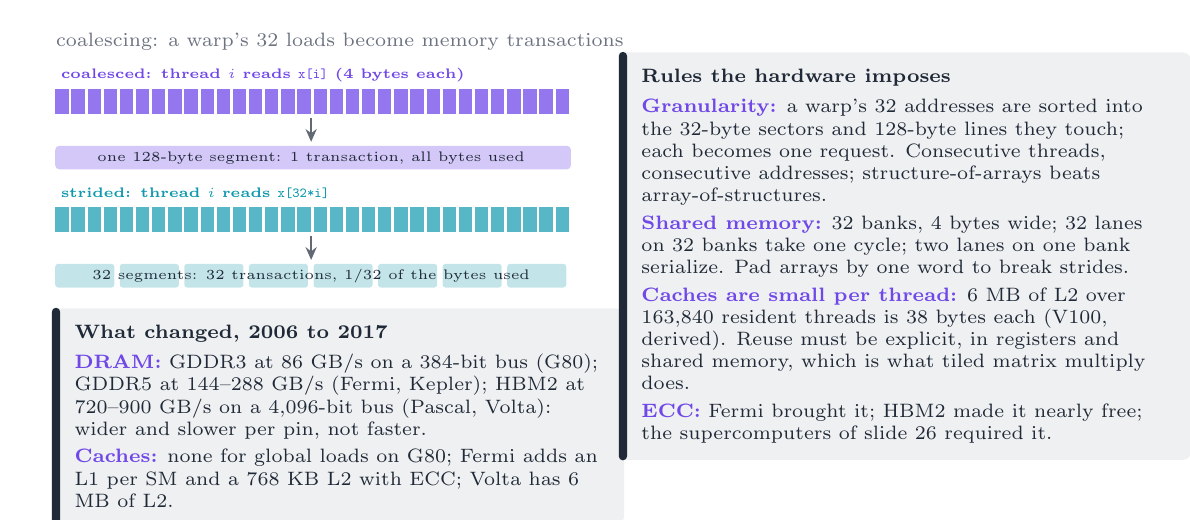
\begin{tikzpicture}
  \useasboundingbox (0,0) rectangle (14.4,5.9);
  \node[lab,anchor=south west] at (0.3,5.55) {coalescing: a warp's 32 loads become memory transactions};
  \begin{scope}[shift={(0.3,3.35)}]
    \node[font=\tiny\bfseries,text=posc,anchor=west] at (0,1.95) {coalesced: thread $i$ reads \texttt{x[i]} (4 bytes each)};
    \foreach \l in {0,...,31}{\fill[posc!75] (0.05+\l*0.205,1.45) rectangle ++(0.17,0.32);}
    \draw[flow] (3.3,1.4) -- (3.3,1.1);
    \fill[posc!30,rounded corners=1.5pt] (0.05,0.75) rectangle (6.6,1.05); \node[font=\tiny,text=ink] at (3.3,0.9) {one 128-byte segment: 1 transaction, all bytes used};
    \node[font=\tiny\bfseries,text=vc,anchor=west] at (0,0.45) {strided: thread $i$ reads \texttt{x[32*i]}};
    \foreach \l in {0,...,31}{\fill[vc!70] (0.05+\l*0.205,-0.05) rectangle ++(0.17,0.32);}
    \draw[flow] (3.3,-0.1) -- (3.3,-0.4);
    \foreach \s in {0,...,7}{\fill[vc!25,rounded corners=1pt] (0.05+\s*0.82,-0.75) rectangle ++(0.75,0.3);}
    \node[font=\tiny,text=ink] at (3.3,-0.6) {32 segments: 32 transactions, 1/32 of the bytes used};
  \end{scope}
  \bgpanels{0.3}{2.35}{6.7cm}{What changed, 2006 to 2017}{%
    \hl{posc}{DRAM:} GDDR3 at 86 GB/s on a 384-bit bus (G80); GDDR5 at
    144--288 GB/s (Fermi, Kepler); HBM2 at 720--900 GB/s on a 4{,}096-bit
    bus (Pascal, Volta): wider and slower per pin, not faster.\\[2pt]
    \hl{posc}{Caches:} none for global loads on G80; Fermi adds an L1
    per SM and a 768 KB L2 with ECC; Volta has 6 MB of L2.}
  \bgpanels{7.5}{5.6}{6.7cm}{Rules the hardware imposes}{%
    \hl{posc}{Granularity:} a warp's 32 addresses are sorted into the
    32-byte sectors and 128-byte lines they touch; each becomes one
    request. Consecutive threads, consecutive addresses;
    structure-of-arrays beats array-of-structures.\\[2pt]
    \hl{posc}{Shared memory:} 32 banks, 4 bytes wide; 32 lanes on 32
    banks take one cycle; two lanes on one bank serialize. Pad arrays
    by one word to break strides.\\[2pt]
    \hl{posc}{Caches are small per thread:} 6 MB of L2 over 163{,}840
    resident threads is 38 bytes each (V100, derived). Reuse must be
    explicit, in registers and shared memory, which is what tiled
    matrix multiply does.\\[2pt]
    \hl{posc}{ECC:} Fermi brought it; HBM2 made it nearly free; the
    supercomputers of slide 26 required it.}
\end{tikzpicture}
\end{frame}

% ---------------------------------------------------------------- 15
\begin{frame}{The roofline: which kernels a GPU can feed}
\framesubtitle{Attainable FLOP/s is the smaller of peak arithmetic and bandwidth times intensity; most kernels sit on the slope.}
\centering
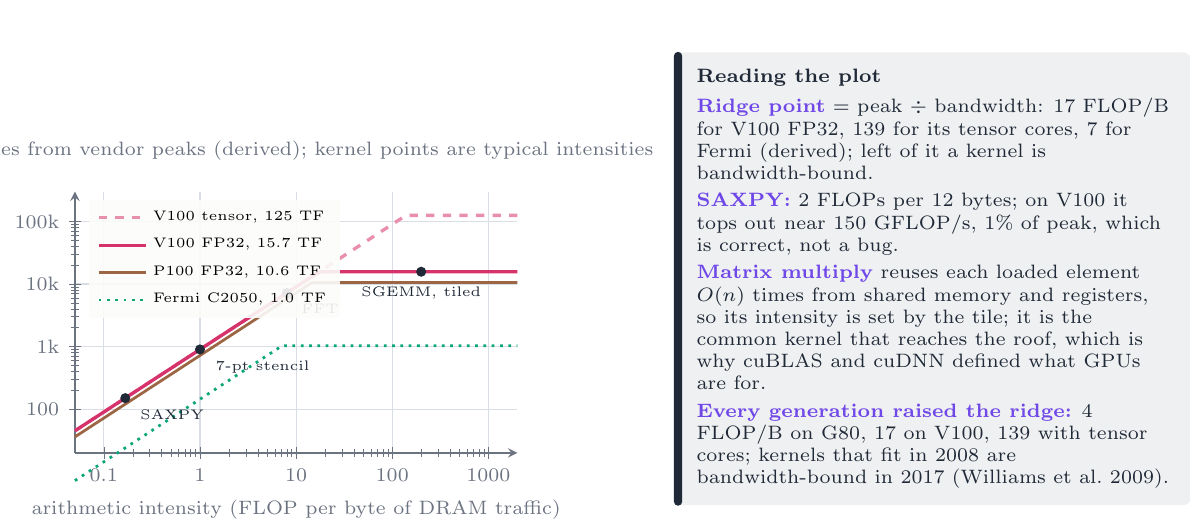
\begin{tikzpicture}
  \useasboundingbox (0,0) rectangle (14.4,5.9);
  \begin{scope}[shift={(0.6,0.5)}]
  \begin{axis}[lecture,width=7.2cm,height=4.9cm,xmode=log,ymode=log,xmin=0.05,xmax=2000,ymin=20,ymax=300000,
      xlabel={arithmetic intensity (FLOP per byte of DRAM traffic)},ylabel={attainable GFLOP/s},
      xtick={0.1,1,10,100,1000},xticklabels={0.1,1,10,100,1000},
      ytick={100,1000,10000,100000},yticklabels={100,1k,10k,100k},
      legend style={at={(0.03,0.97)},anchor=north west,font=\tiny,fill=paper,fill opacity=0.9,text opacity=1},
      title style={font=\scriptsize,text=muted,at={(0.5,1.02)}},title={rooflines from vendor peaks (derived); kernel points are typical intensities}]
    \addplot[outc!55,line width=1.2pt,dashed,domain=0.05:2000,samples=100] {min(125000, 900*x)};
    \addlegendentry{V100 tensor, 125 TF}
    \addplot[outc,line width=1.2pt,domain=0.05:2000,samples=100] {min(15700, 900*x)};
    \addlegendentry{V100 FP32, 15.7 TF}
    \addplot[trn,line width=1.0pt,domain=0.05:2000,samples=100] {min(10600, 720*x)};
    \addlegendentry{P100 FP32, 10.6 TF}
    \addplot[emb,line width=1.0pt,dotted,domain=0.05:2000,samples=100] {min(1030, 144*x)};
    \addlegendentry{Fermi C2050, 1.0 TF}
    \addplot[only marks,mark=*,mark size=1.6pt,ink] coordinates {(0.167,150) (1,900) (8,7200) (200,15700)};
    \node[font=\tiny,text=ink,anchor=north west] at (axis cs:0.19,140) {SAXPY};
    \node[font=\tiny,text=ink,anchor=north west] at (axis cs:1.15,850) {7-pt stencil};
    \node[font=\tiny,text=ink,anchor=north west] at (axis cs:9,6800) {FFT};
    \node[font=\tiny,text=ink,anchor=north] at (axis cs:200,13000) {SGEMM, tiled};
  \end{axis}
  \end{scope}
  \bgpanels{8.2}{5.6}{6.0cm}{Reading the plot}{%
    \hl{posc}{Ridge point} $=$ peak $\div$ bandwidth: 17 FLOP/B for
    V100 FP32, 139 for its tensor cores, 7 for Fermi (derived); left
    of it a kernel is bandwidth-bound.\\[2pt]
    \hl{posc}{SAXPY:} 2 FLOPs per 12 bytes; on V100 it tops out near
    150 GFLOP/s, 1\% of peak, which is correct, not a bug.\\[2pt]
    \hl{posc}{Matrix multiply} reuses each loaded element $O(n)$ times
    from shared memory and registers, so its intensity is set by the
    tile; it is the common kernel that reaches the roof, which is why
    cuBLAS and cuDNN defined what GPUs are for.\\[2pt]
    \hl{posc}{Every generation raised the ridge:} 4 FLOP/B on G80, 17
    on V100, 139 with tensor cores; kernels that fit in 2008 are
    bandwidth-bound in 2017 (Williams et al.\ 2009).}
\end{tikzpicture}
\end{frame}

% ---------------------------------------------------------------- 16
\stage{7}
\begin{frame}{Tesla to Fermi (2008--2010): double precision, caches, ECC}
\framesubtitle{GT200 made the GPU usable for science; Fermi made it a general processor and put it at the top of the TOP500.}
\centering
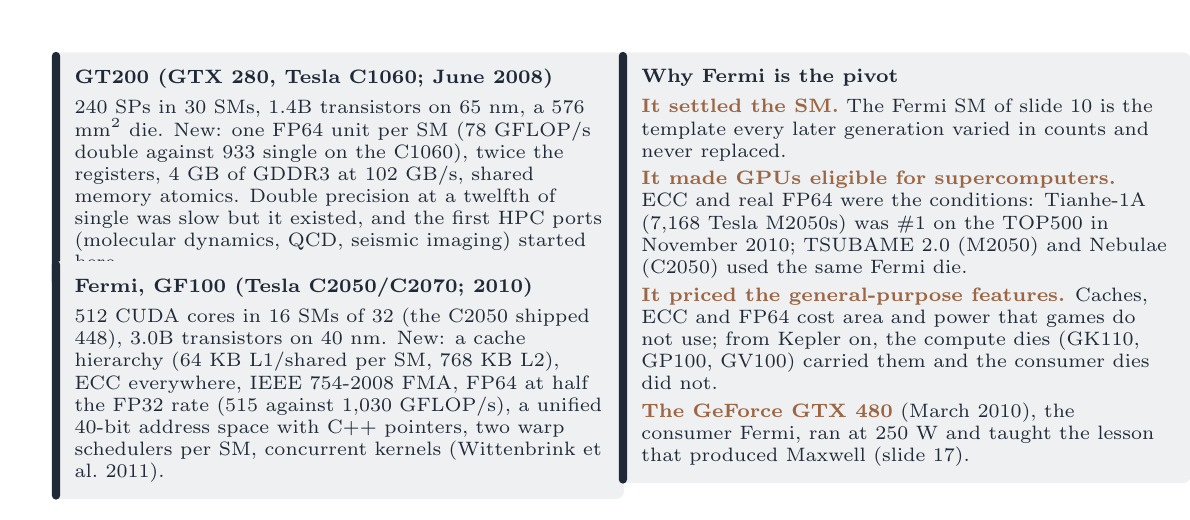
\begin{tikzpicture}
  \useasboundingbox (0,0) rectangle (14.4,5.9);
  \bgpanels{0.3}{5.6}{6.7cm}{GT200 (GTX 280, Tesla C1060; June 2008)}{%
    240 SPs in 30 SMs, 1.4B transistors on 65 nm, a 576 mm$^2$ die.
    New: one FP64 unit per SM (78 GFLOP/s double against 933 single on
    the C1060), twice the registers, 4 GB of GDDR3 at 102 GB/s, shared
    memory atomics. Double precision at a twelfth of single was slow
    but it existed, and the first HPC ports (molecular dynamics, QCD,
    seismic imaging) started here.}
  \bgpanels{0.3}{2.95}{6.7cm}{Fermi, GF100 (Tesla C2050/C2070; 2010)}{%
    512 CUDA cores in 16 SMs of 32 (the C2050 shipped 448), 3.0B
    transistors on 40 nm. New: a cache hierarchy (64 KB L1/shared per
    SM, 768 KB L2), ECC everywhere, IEEE 754-2008 FMA, FP64 at half the
    FP32 rate (515 against 1{,}030 GFLOP/s), a unified 40-bit address
    space with C++ pointers, two warp schedulers per SM, concurrent
    kernels (Wittenbrink et al.\ 2011).}
  \bgpanels{7.5}{5.6}{6.7cm}{Why Fermi is the pivot}{%
    \hl{trn}{It settled the SM.} The Fermi SM of slide 10 is the
    template every later generation varied in counts and never
    replaced.\\[2pt]
    \hl{trn}{It made GPUs eligible for supercomputers.} ECC and real
    FP64 were the conditions: Tianhe-1A (7{,}168 Tesla M2050s) was \#1
    on the TOP500 in November 2010; TSUBAME 2.0 (M2050) and Nebulae
    (C2050) used the same Fermi die.\\[2pt]
    \hl{trn}{It priced the general-purpose features.} Caches, ECC and
    FP64 cost area and power that games do not use; from Kepler on,
    the compute dies (GK110, GP100, GV100) carried them and the
    consumer dies did not.\\[2pt]
    \hl{trn}{The GeForce GTX 480} (March 2010), the consumer Fermi,
    ran at 250 W and taught the lesson that produced Maxwell (slide
    17).}
\end{tikzpicture}
\end{frame}

% ---------------------------------------------------------------- 17
\begin{frame}{Kepler and Maxwell (2012--2015): wider SMs, then efficiency}
\framesubtitle{Kepler put 192 lanes in an SM and 18{,}688 GPUs in Titan; Maxwell cut back to 128 lanes and doubled perf per watt$^\dagger$.}
\centering
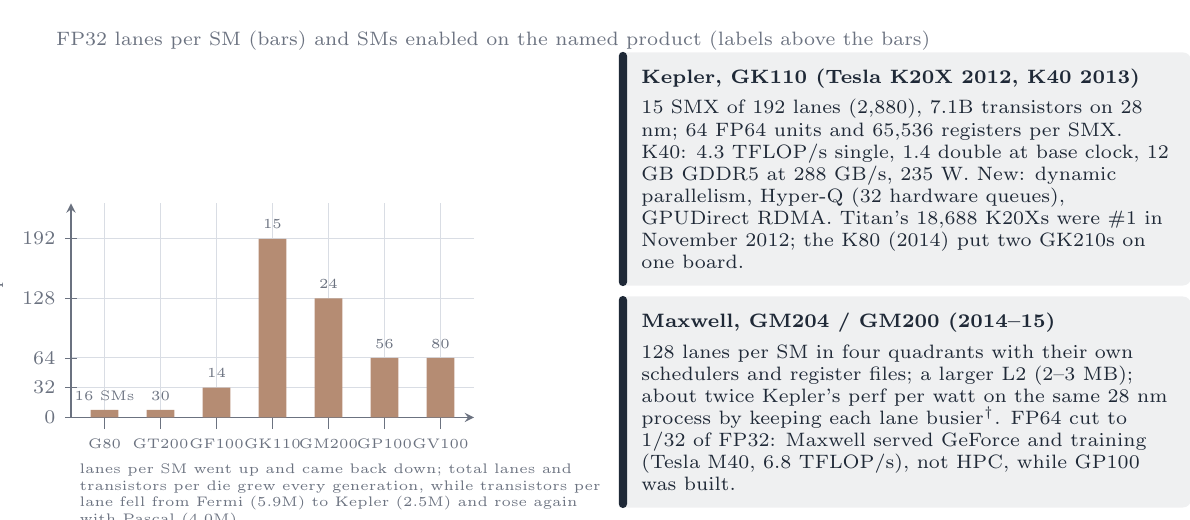
\begin{tikzpicture}
  \useasboundingbox (0,0) rectangle (14.4,5.9);
  \node[lab,anchor=south west] at (0.3,5.55) {FP32 lanes per SM (bars) and SMs enabled on the named product (labels above the bars)};
  \begin{scope}[shift={(0.55,0.95)}]
  \begin{axis}[lecture,width=6.7cm,height=4.3cm,ybar,bar width=10pt,enlarge x limits=0.1,ymin=0,ymax=230,
      symbolic x coords={G80,GT200,GF100,GK110,GM200,GP100,GV100},xtick=data,xticklabel style={font=\tiny},
      ylabel={FP32 lanes per SM},ytick={0,32,64,128,192},
      nodes near coords,nodes near coords style={font=\tiny,text=muted},
      point meta=explicit symbolic]
    \addplot[fill=trn!75,draw=none] coordinates {(G80,8)[16 SMs] (GT200,8)[30] (GF100,32)[14] (GK110,192)[15] (GM200,128)[24] (GP100,64)[56] (GV100,64)[80]};
  \end{axis}
  \end{scope}
  \node[lab,font=\tiny,anchor=north west,text width=6.7cm] at (0.6,0.42) {lanes per SM went up and came back down; total lanes and transistors per die grew every generation, while transistors per lane fell from Fermi (5.9M) to Kepler (2.5M) and rose again with Pascal (4.0M)};
  \bgpanels{7.5}{5.6}{6.7cm}{Kepler, GK110 (Tesla K20X 2012, K40 2013)}{%
    15 SMX of 192 lanes (2{,}880), 7.1B transistors on 28 nm; 64 FP64
    units and 65{,}536 registers per SMX. K40: 4.3 TFLOP/s single, 1.4
    double at base clock, 12 GB GDDR5 at 288 GB/s, 235 W. New: dynamic
    parallelism, Hyper-Q (32 hardware queues), GPUDirect RDMA. Titan's
    18{,}688 K20Xs were \#1 in November 2012; the K80 (2014) put two
    GK210s on one board.}
  \bgpanels{7.5}{2.5}{6.7cm}{Maxwell, GM204 / GM200 (2014--15)}{%
    128 lanes per SM in four quadrants with their own schedulers and
    register files; a larger L2 (2--3 MB); about twice Kepler's perf
    per watt on the same 28 nm process by keeping each lane
    busier$^\dagger$. FP64 cut to 1/32 of FP32: Maxwell served GeForce
    and training (Tesla M40, 6.8 TFLOP/s), not HPC, while GP100 was
    built.}
\end{tikzpicture}
\end{frame}

% ---------------------------------------------------------------- 18
\begin{frame}{The generations in one table}
\framesubtitle{Seven compute dies, 2006--2017: the counts change by an order of magnitude; the structure does not.}
\centering
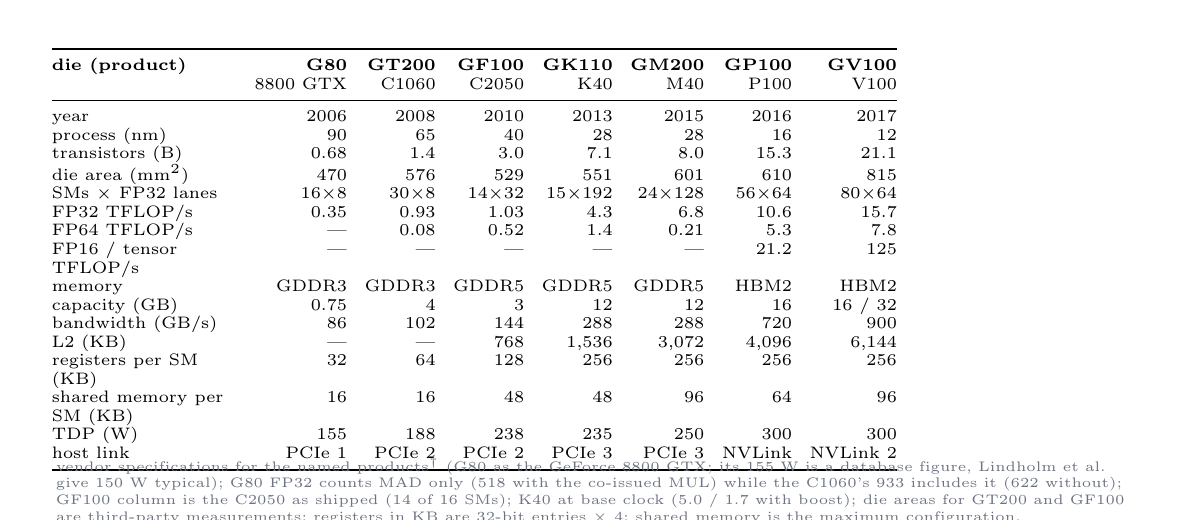
\begin{tikzpicture}
  \useasboundingbox (0,0) rectangle (14.4,5.9);
  \node[anchor=north west,inner sep=0,font=\fontsize{5.7}{6.7}\selectfont] at (0.3,5.65) {%
    \renewcommand{\arraystretch}{1.0}\setlength{\tabcolsep}{3.2pt}%
    \begin{tabular}{@{}>{\raggedright\arraybackslash}p{2.35cm}rrrrrrr@{}}
      \toprule
      \textbf{die (product)} & \textbf{G80} & \textbf{GT200} & \textbf{GF100} & \textbf{GK110} & \textbf{GM200} & \textbf{GP100} & \textbf{GV100}\\
       & 8800 GTX & C1060 & C2050 & K40 & M40 & P100 & V100\\
      \midrule
      year & 2006 & 2008 & 2010 & 2013 & 2015 & 2016 & 2017\\
      process (nm) & 90 & 65 & 40 & 28 & 28 & 16 & 12\\
      transistors (B) & 0.68 & 1.4 & 3.0 & 7.1 & 8.0 & 15.3 & 21.1\\
      die area (mm$^2$) & 470 & 576 & 529 & 551 & 601 & 610 & 815\\
      SMs $\times$ FP32 lanes & 16$\times$8 & 30$\times$8 & 14$\times$32 & 15$\times$192 & 24$\times$128 & 56$\times$64 & 80$\times$64\\
      FP32 TFLOP/s & 0.35 & 0.93 & 1.03 & 4.3 & 6.8 & 10.6 & 15.7\\
      FP64 TFLOP/s & --- & 0.08 & 0.52 & 1.4 & 0.21 & 5.3 & 7.8\\
      FP16 / tensor TFLOP/s & --- & --- & --- & --- & --- & 21.2 & 125\\
      memory & GDDR3 & GDDR3 & GDDR5 & GDDR5 & GDDR5 & HBM2 & HBM2\\
      capacity (GB) & 0.75 & 4 & 3 & 12 & 12 & 16 & 16 / 32\\
      bandwidth (GB/s) & 86 & 102 & 144 & 288 & 288 & 720 & 900\\
      L2 (KB) & --- & --- & 768 & 1{,}536 & 3{,}072 & 4{,}096 & 6{,}144\\
      registers per SM (KB) & 32 & 64 & 128 & 256 & 256 & 256 & 256\\
      shared memory per SM (KB) & 16 & 16 & 48 & 48 & 96 & 64 & 96\\
      TDP (W) & 155 & 188 & 238 & 235 & 250 & 300 & 300\\
      host link & PCIe 1 & PCIe 2 & PCIe 2 & PCIe 3 & PCIe 3 & NVLink & NVLink 2\\
      \bottomrule
    \end{tabular}};
  \node[lab,anchor=north west,text width=13.8cm,font=\tiny] at (0.3,0.52) {vendor specifications for the named products$^\dagger$ (G80 as the GeForce 8800 GTX; its 155 W is a database figure, Lindholm et al.\ give 150 W typical); G80 FP32 counts MAD only (518 with the co-issued MUL) while the C1060's 933 includes it (622 without); GF100 column is the C2050 as shipped (14 of 16 SMs); K40 at base clock (5.0 / 1.7 with boost); die areas for GT200 and GF100 are third-party measurements; registers in KB are 32-bit entries $\times$ 4; shared memory is the maximum configuration.};
\end{tikzpicture}
\end{frame}

% ---------------------------------------------------------------- 19
\begin{frame}{Deep learning arrives (2012--2016) and the architecture answers}
\framesubtitle{AlexNet trained on two GeForce cards; five years later the compute die had a unit for nothing but matrix multiply.}
\centering
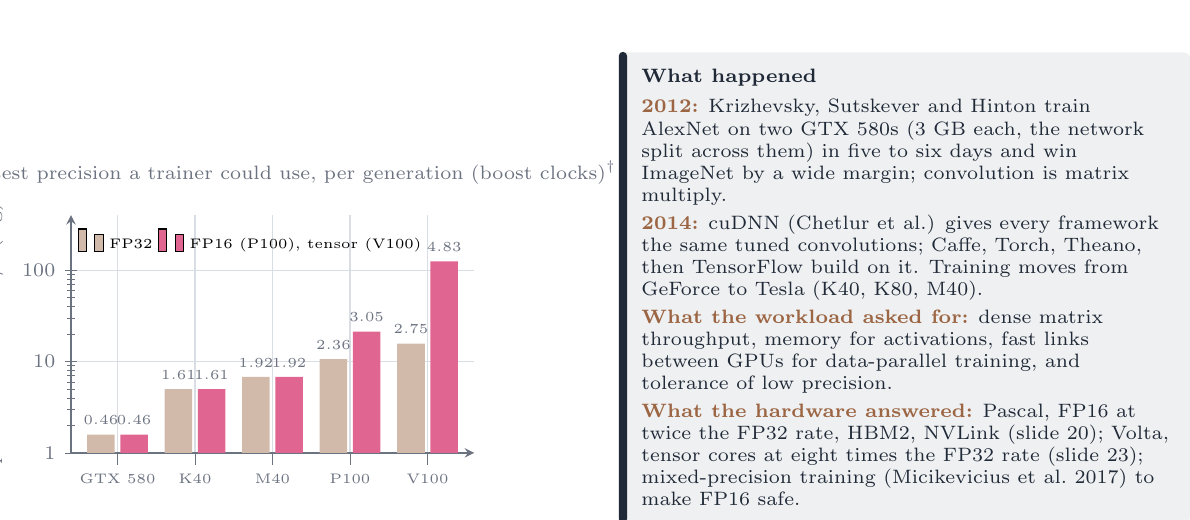
\begin{tikzpicture}
  \useasboundingbox (0,0) rectangle (14.4,5.9);
  \begin{scope}[shift={(0.55,0.5)}]
  \begin{axis}[lecture,width=6.7cm,height=4.6cm,ybar,bar width=10pt,ymode=log,ymin=1,ymax=400,enlarge x limits=0.15,
      symbolic x coords={GTX 580,K40,M40,P100,V100},xtick=data,xticklabel style={font=\tiny},
      ylabel={peak dense TFLOP/s (log)},ytick={1,10,100},yticklabels={1,10,100},
      nodes near coords,nodes near coords style={font=\tiny,text=muted},
      title style={font=\scriptsize,text=muted,at={(0.5,1.02)}},title={the fastest precision a trainer could use, per generation (boost clocks)$^\dagger$},
      legend style={at={(0.45,0.97)},anchor=north,font=\tiny,legend columns=2}]
    \addplot[fill=trn!45,draw=none] coordinates {(GTX 580,1.58) (K40,5.0) (M40,6.8) (P100,10.6) (V100,15.7)};
    \addlegendentry{FP32}
    \addplot[fill=outc!75,draw=none] coordinates {(GTX 580,1.58) (K40,5.0) (M40,6.8) (P100,21.2) (V100,125)};
    \addlegendentry{FP16 (P100), tensor (V100)}
  \end{axis}
  \end{scope}
  \bgpanels{7.5}{5.6}{6.7cm}{What happened}{%
    \hl{trn}{2012:} Krizhevsky, Sutskever and Hinton train AlexNet on
    two GTX 580s (3 GB each, the network split across them) in five to
    six days and win ImageNet by a wide margin; convolution is matrix
    multiply.\\[2pt]
    \hl{trn}{2014:} cuDNN (Chetlur et al.) gives every framework the
    same tuned convolutions; Caffe, Torch, Theano, then TensorFlow build
    on it. Training moves from GeForce to Tesla (K40, K80, M40).\\[2pt]
    \hl{trn}{What the workload asked for:} dense matrix throughput,
    memory for activations, fast links between GPUs for data-parallel
    training, and tolerance of low precision.\\[2pt]
    \hl{trn}{What the hardware answered:} Pascal, FP16 at twice the
    FP32 rate, HBM2, NVLink (slide 20); Volta, tensor cores at eight
    times the FP32 rate (slide 23); mixed-precision training
    (Micikevicius et al.\ 2017) to make FP16 safe.}
\end{tikzpicture}
\end{frame}

% ---------------------------------------------------------------- 20
\begin{frame}{Pascal GP100 (2016): 16 nm FinFET, HBM2, NVLink}
\framesubtitle{The first compute die built for deep learning as well as HPC: 15.3B transistors, 720 GB/s, FP16 at double rate, NVLink.}
\centering
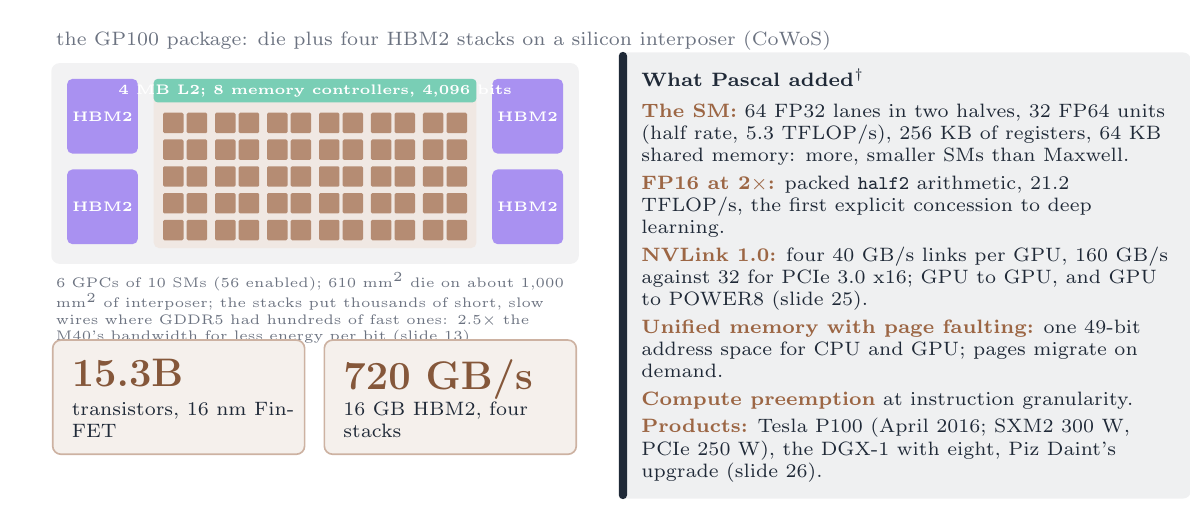
\begin{tikzpicture}
  \useasboundingbox (0,0) rectangle (14.4,5.9);
  \node[lab,anchor=south west] at (0.3,5.55) {the GP100 package: die plus four HBM2 stacks on a silicon interposer (CoWoS)};
  \begin{scope}[shift={(0.3,2.9)}]
    \fill[ink!6,rounded corners=3pt] (0,0) rectangle (6.7,2.55);
    \foreach \s in {0,1}{\fill[posc!60,rounded corners=2pt] (0.2,0.25+\s*1.15) rectangle ++(0.9,0.95); \node[font=\tiny\bfseries,text=white] at (0.65,0.72+\s*1.15) {HBM2};
      \fill[posc!60,rounded corners=2pt] (5.6,0.25+\s*1.15) rectangle ++(0.9,0.95); \node[font=\tiny\bfseries,text=white] at (6.05,0.72+\s*1.15) {HBM2};}
    \fill[trn!15,rounded corners=2pt] (1.3,0.2) rectangle (5.4,2.35);
    \foreach \g in {0,...,5}{\foreach \r in {0,...,9}{\fill[trn!75,rounded corners=0.5pt] ({1.42+\g*0.66+mod(\r,2)*0.3},{0.3+floor(\r/2)*0.34}) rectangle ++(0.26,0.26);}}
    \fill[emb!55,rounded corners=1.5pt] (1.3,2.05) rectangle (5.4,2.35); \node[font=\tiny\bfseries,text=white] at (3.35,2.2) {4 MB L2; 8 memory controllers, 4{,}096 bits};
  \end{scope}
  \node[lab,font=\tiny,anchor=north west,text width=6.7cm] at (0.3,2.85) {6 GPCs of 10 SMs (56 enabled); 610 mm$^2$ die on about 1{,}000 mm$^2$ of interposer; the stacks put thousands of short, slow wires where GDDR5 had hundreds of fast ones: 2.5$\times$ the M40's bandwidth for less energy per bit (slide 13)};
  \stat{0.3}{1.95}{15.3B}{transistors, 16 nm FinFET}{trn}
  \stat{3.75}{1.95}{720 GB/s}{16 GB HBM2, four stacks}{trn}
  \bgpanels{7.5}{5.6}{6.7cm}{What Pascal added$^\dagger$}{%
    \hl{trn}{The SM:} 64 FP32 lanes in two halves, 32 FP64 units (half
    rate, 5.3 TFLOP/s), 256 KB of registers, 64 KB shared memory:
    more, smaller SMs than Maxwell.\\[2pt]
    \hl{trn}{FP16 at 2$\times$:} packed \texttt{half2} arithmetic, 21.2
    TFLOP/s, the first explicit concession to deep learning.\\[2pt]
    \hl{trn}{NVLink 1.0:} four 40 GB/s links per GPU, 160 GB/s against
    32 for PCIe 3.0 x16; GPU to GPU, and GPU to POWER8 (slide 25).\\[2pt]
    \hl{trn}{Unified memory with page faulting:} one 49-bit address
    space for CPU and GPU; pages migrate on demand.\\[2pt]
    \hl{trn}{Compute preemption} at instruction granularity.\\[2pt]
    \hl{trn}{Products:} Tesla P100 (April 2016; SXM2 300 W, PCIe 250
    W), the DGX-1 with eight, Piz Daint's upgrade (slide 26).}
\end{tikzpicture}
\end{frame}

% ---------------------------------------------------------------- 21
\begin{frame}{Reading a Pascal or Volta SM: four schedulers, many lanes}
\framesubtitle{The SM is partitioned into quarters, each with its own scheduler and registers; the whole shares L1 and shared memory.}
\centering
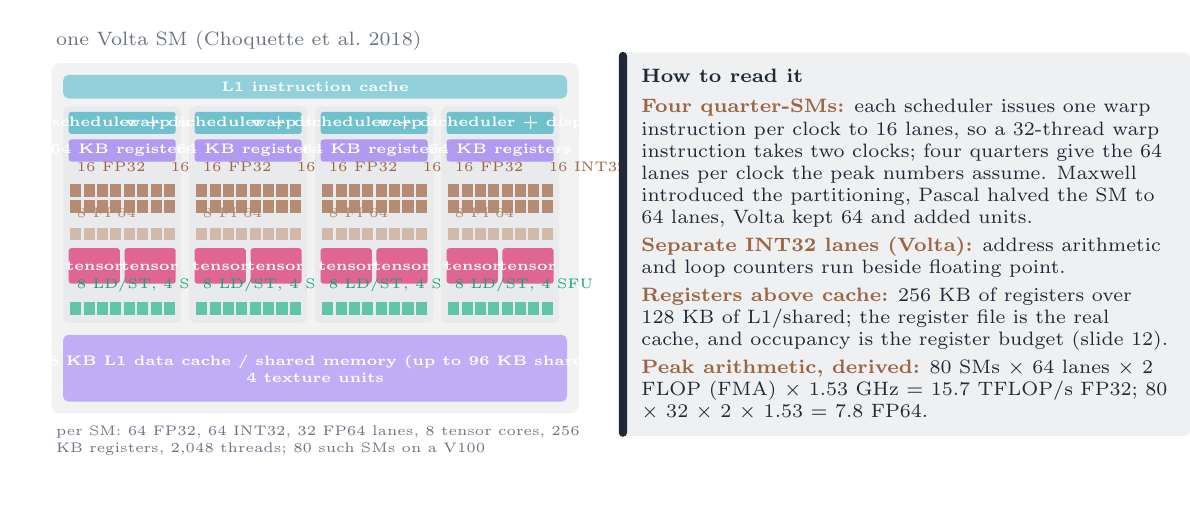
\begin{tikzpicture}
  \useasboundingbox (0,0) rectangle (14.4,5.9);
  \node[lab,anchor=south west] at (0.3,5.55) {one Volta SM (Choquette et al.\ 2018)};
  \begin{scope}[shift={(0.3,1.0)}]
    \fill[ink!6,rounded corners=3pt] (0,0) rectangle (6.7,4.45);
    \fill[vc!45,rounded corners=2pt] (0.15,4.0) rectangle (6.55,4.3); \node[font=\tiny\bfseries,text=white] at (3.35,4.15) {L1 instruction cache};
    \foreach \q in {0,...,3}{
      \begin{scope}[shift={(0.15+\q*1.6,1.15)}]
        \fill[ink!10,rounded corners=2pt] (0,0) rectangle (1.5,2.75);
        \fill[vc!60,rounded corners=1pt] (0.07,2.4) rectangle (1.43,2.68); \node[font=\fontsize{4.5}{5}\selectfont\bfseries,text=white] at (0.75,2.54) {warp scheduler + dispatch};
        \fill[posc!55,rounded corners=1pt] (0.07,2.05) rectangle (1.43,2.33); \node[font=\fontsize{4.5}{5}\selectfont\bfseries,text=white] at (0.75,2.19) {64 KB registers};
        \foreach \r in {0,1}{\foreach \c in {0,...,7}{\fill[trn!75] (0.09+\c*0.17,1.6-\r*0.2) rectangle ++(0.14,0.16);}}
        \node[font=\fontsize{4.5}{5}\selectfont,text=trn,anchor=south west] at (0.05,1.8) {16 FP32 \quad 16 INT32};
        \foreach \c in {0,...,7}{\fill[trn!45] (0.09+\c*0.17,1.05) rectangle ++(0.14,0.16);}
        \node[font=\fontsize{4.5}{5}\selectfont,text=trn!80,anchor=south west] at (0.05,1.22) {8 FP64};
        \fill[outc!75,rounded corners=1pt] (0.07,0.5) rectangle (0.72,0.95); \fill[outc!75,rounded corners=1pt] (0.78,0.5) rectangle (1.43,0.95);
        \node[font=\fontsize{4.5}{5}\selectfont\bfseries,text=white] at (0.4,0.72) {tensor}; \node[font=\fontsize{4.5}{5}\selectfont\bfseries,text=white] at (1.1,0.72) {tensor};
        \foreach \c in {0,...,7}{\fill[emb!65] (0.09+\c*0.17,0.1) rectangle ++(0.14,0.16);} \node[font=\fontsize{4.5}{5}\selectfont,text=emb,anchor=south west] at (0.05,0.27) {8 LD/ST, 4 SFU};
      \end{scope}}
    \fill[posc!45,rounded corners=2pt] (0.15,0.15) rectangle (6.55,1.0);
    \node[font=\tiny\bfseries,text=white,align=center] at (3.35,0.57) {128 KB L1 data cache / shared memory (up to 96 KB shared)\\ 4 texture units};
  \end{scope}
  \node[lab,font=\tiny,anchor=north west,text width=6.7cm] at (0.3,0.9) {per SM: 64 FP32, 64 INT32, 32 FP64 lanes, 8 tensor cores, 256 KB registers, 2{,}048 threads; 80 such SMs on a V100};
  \bgpanels{7.5}{5.6}{6.7cm}{How to read it}{%
    \hl{trn}{Four quarter-SMs:} each scheduler issues one warp
    instruction per clock to 16 lanes, so a 32-thread warp instruction
    takes two clocks; four quarters give the 64 lanes per clock the
    peak numbers assume. Maxwell introduced the partitioning, Pascal
    halved the SM to 64 lanes, Volta kept 64 and added units.\\[2pt]
    \hl{trn}{Separate INT32 lanes (Volta):} address arithmetic and loop
    counters run beside floating point.\\[2pt]
    \hl{trn}{Registers above cache:} 256 KB of registers over 128 KB
    of L1/shared; the register file is the real cache, and occupancy
    is the register budget (slide 12).\\[2pt]
    \hl{trn}{Peak arithmetic, derived:} 80 SMs $\times$ 64 lanes
    $\times$ 2 FLOP (FMA) $\times$ 1.53 GHz $=$ 15.7 TFLOP/s FP32; 80
    $\times$ 32 $\times$ 2 $\times$ 1.53 $=$ 7.8 FP64.}
\end{tikzpicture}
\end{frame}

% ---------------------------------------------------------------- 22
\stage{8}
\begin{frame}{Volta GV100 (2017): the largest die, and a new kind of unit}
\framesubtitle{21.1 billion transistors on 815 mm$^2$, near the reticle limit; 80 SMs, 640 tensor cores, 900 GB/s of HBM2, NVLink 2.}
\centering
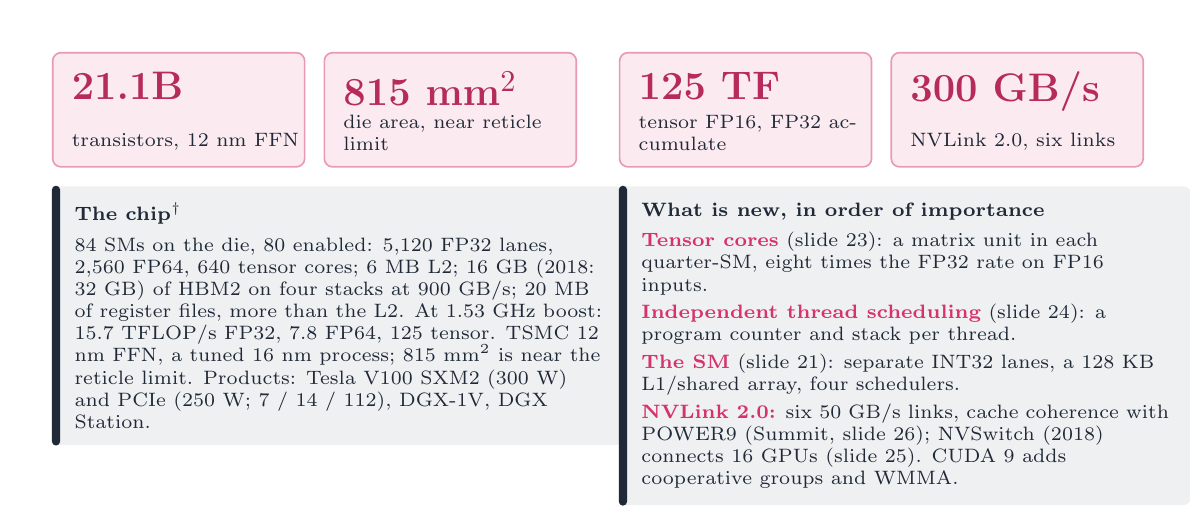
\begin{tikzpicture}
  \useasboundingbox (0,0) rectangle (14.4,5.9);
  \stat{0.3}{5.6}{21.1B}{transistors, 12 nm FFN}{outc}
  \stat{3.75}{5.6}{815 mm$^2$}{die area, near reticle limit}{outc}
  \stat{7.5}{5.6}{125 TF}{tensor FP16, FP32 accumulate}{outc}
  \stat{10.95}{5.6}{300 GB/s}{NVLink 2.0, six links}{outc}
  \bgpanels{0.3}{3.9}{6.7cm}{The chip$^\dagger$}{%
    84 SMs on the die, 80 enabled: 5{,}120 FP32 lanes, 2{,}560 FP64,
    640 tensor cores; 6 MB L2; 16 GB (2018: 32 GB) of HBM2 on four
    stacks at 900 GB/s; 20 MB of register files, more than the L2. At
    1.53 GHz boost: 15.7 TFLOP/s FP32, 7.8 FP64, 125 tensor. TSMC 12
    nm FFN, a tuned 16 nm process; 815 mm$^2$ is near the reticle limit.
    Products: Tesla V100 SXM2 (300 W) and PCIe (250 W; 7 / 14 / 112),
    DGX-1V, DGX Station.}
  \bgpanels{7.5}{3.9}{6.7cm}{What is new, in order of importance}{%
    \hl{outc}{Tensor cores} (slide 23): a matrix unit in each
    quarter-SM, eight times the FP32 rate on FP16 inputs.\\[2pt]
    \hl{outc}{Independent thread scheduling} (slide 24): a program
    counter and stack per thread.\\[2pt]
    \hl{outc}{The SM} (slide 21): separate INT32 lanes, a 128 KB
    L1/shared array, four schedulers.\\[2pt]
    \hl{outc}{NVLink 2.0:} six 50 GB/s links, cache coherence with
    POWER9 (Summit, slide 26); NVSwitch (2018) connects 16 GPUs
    (slide 25). CUDA 9 adds cooperative groups and WMMA.}
\end{tikzpicture}
\end{frame}

% ---------------------------------------------------------------- 23
\begin{frame}{Tensor cores: a 4$\times$4$\times$4 matrix multiply-add per clock}
\framesubtitle{$D = A B + C$ on 4$\times$4 tiles, FP16 in and FP32 out: 64 fused multiply-adds per clock per tensor core, 512 per SM.}
\centering
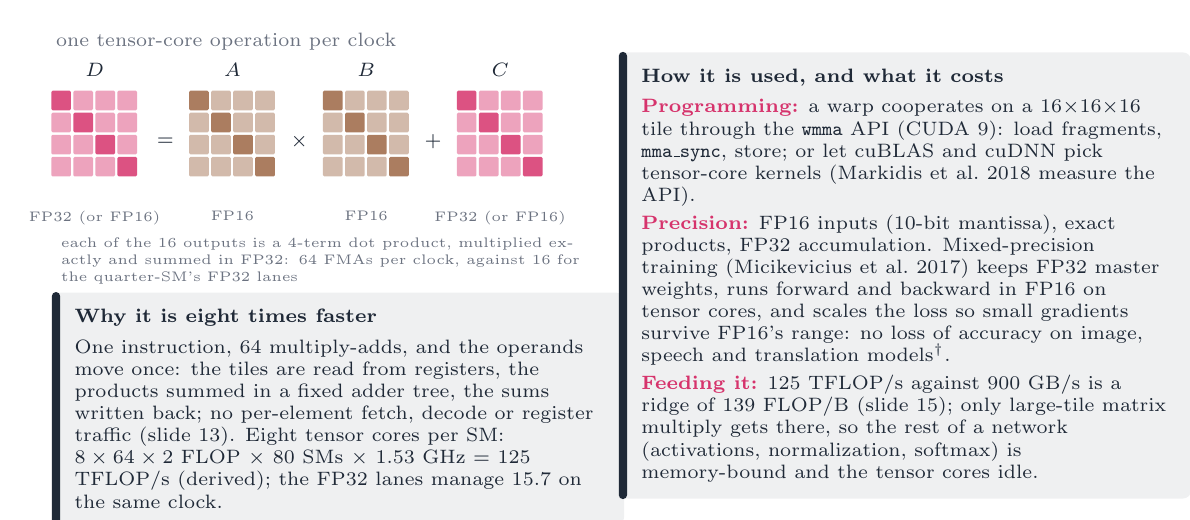
\begin{tikzpicture}
  \useasboundingbox (0,0) rectangle (14.4,5.9);
  \node[lab,anchor=south west] at (0.3,5.55) {one tensor-core operation per clock};
  \begin{scope}[shift={(0.3,3.3)}]
    \foreach \m/\x/\c/\lbl in {D/0.0/outc/{FP32 (or FP16)}, A/1.75/trn/{FP16}, B/3.45/trn/{FP16}, C/5.15/outc/{FP32 (or FP16)}}{
      \foreach \r in {0,...,3}{\foreach \k in {0,...,3}{\pgfmathtruncatemacro{\sh}{(\r==\k)?85:45}\fill[\c!\sh,rounded corners=0.5pt] (\x+\k*0.28,1.55-\r*0.28) rectangle ++(0.25,0.25);}}
      \node[font=\scriptsize\bfseries,text=ink,anchor=south] at (\x+0.55,1.85) {$\m$};
      \node[font=\tiny,text=muted,anchor=north] at (\x+0.55,0.4) {\lbl};}
    \node[font=\scriptsize,text=ink] at (1.45,1.15) {$=$};
    \node[font=\scriptsize,text=ink] at (3.15,1.15) {$\times$};
    \node[font=\scriptsize,text=ink] at (4.85,1.15) {$+$};
    \node[font=\tiny,text=muted,anchor=north west,text width=6.6cm] at (0,0.05) {each of the 16 outputs is a 4-term dot product, multiplied exactly and summed in FP32: 64 FMAs per clock, against 16 for the quarter-SM's FP32 lanes};
  \end{scope}
  \bgpanels{0.3}{2.55}{6.7cm}{Why it is eight times faster}{%
    One instruction, 64 multiply-adds, and the operands move once: the
    tiles are read from registers, the products summed in a fixed
    adder tree, the sums written back; no per-element fetch, decode or
    register traffic (slide 13). Eight tensor cores per SM: $8\times
    64\times 2$ FLOP $\times$ 80 SMs $\times$ 1.53 GHz $=$ 125 TFLOP/s
    (derived); the FP32 lanes manage 15.7 on the same clock.}
  \bgpanels{7.5}{5.6}{6.7cm}{How it is used, and what it costs}{%
    \hl{outc}{Programming:} a warp cooperates on a 16$\times$16$\times$16
    tile through the \texttt{wmma} API (CUDA 9): load fragments,
    \texttt{mma\_sync}, store; or let cuBLAS and cuDNN pick tensor-core
    kernels (Markidis et al.\ 2018 measure the API).\\[2pt]
    \hl{outc}{Precision:} FP16 inputs (10-bit mantissa), exact products,
    FP32 accumulation. Mixed-precision training (Micikevicius et al.\
    2017) keeps FP32 master weights, runs forward and backward in FP16
    on tensor cores, and scales the loss so small gradients survive
    FP16's range: no loss of accuracy on image, speech and translation
    models$^\dagger$.\\[2pt]
    \hl{outc}{Feeding it:} 125 TFLOP/s against 900 GB/s is a ridge of
    139 FLOP/B (slide 15); only large-tile matrix multiply gets there,
    so the rest of a network (activations, normalization, softmax) is
    memory-bound and the tensor cores idle.}
\end{tikzpicture}
\end{frame}

% ---------------------------------------------------------------- 24
\begin{frame}{Independent threads, and what microbenchmarks measure}
\framesubtitle{Volta gives each thread a program counter; measured latencies show where the cycles go in a modern SM.}
\centering
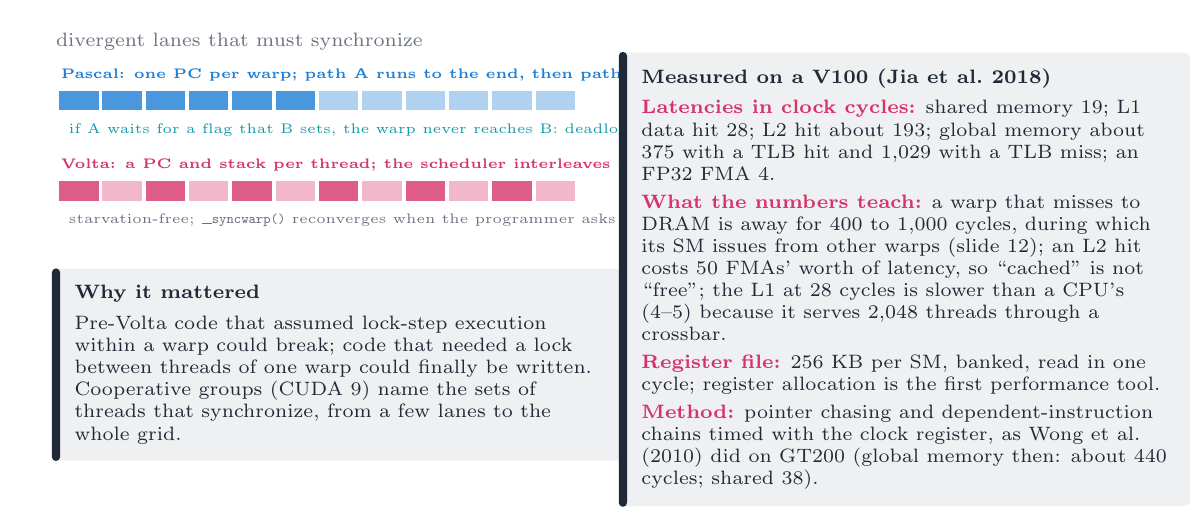
\begin{tikzpicture}
  \useasboundingbox (0,0) rectangle (14.4,5.9);
  \node[lab,anchor=south west] at (0.3,5.55) {divergent lanes that must synchronize};
  \begin{scope}[shift={(0.3,3.55)}]
    \node[font=\tiny\bfseries,text=mlp,anchor=west] at (0,1.75) {Pascal: one PC per warp; path A runs to the end, then path B};
    \foreach \t in {0,...,5}{\fill[mlp!80] (0.1+\t*0.55,1.3) rectangle ++(0.5,0.25);} \foreach \t in {6,...,11}{\fill[mlp!35] (0.1+\t*0.55,1.3) rectangle ++(0.5,0.25);}
    \node[font=\tiny,text=vc,anchor=west] at (0.1,1.05) {if A waits for a flag that B sets, the warp never reaches B: deadlock};
    \node[font=\tiny\bfseries,text=outc,anchor=west] at (0,0.6) {Volta: a PC and stack per thread; the scheduler interleaves A and B};
    \foreach \t in {0,...,11}{\pgfmathtruncatemacro{\sh}{mod(\t,2)==0?80:35}\fill[outc!\sh] (0.1+\t*0.55,0.15) rectangle ++(0.5,0.25);}
    \node[font=\tiny,text=muted,anchor=west] at (0.1,-0.1) {starvation-free; \texttt{\_\_syncwarp()} reconverges when the programmer asks};
  \end{scope}
  \bgpanels{0.3}{2.85}{6.7cm}{Why it mattered}{%
    Pre-Volta code that assumed lock-step execution within a warp
    could break; code that needed a lock between threads of one warp
    could finally be written. Cooperative groups (CUDA 9) name the
    sets of threads that synchronize, from a few lanes to the whole
    grid.}
  \bgpanels{7.5}{5.6}{6.7cm}{Measured on a V100 (Jia et al.\ 2018)}{%
    \hl{outc}{Latencies in clock cycles:} shared memory 19; L1 data
    hit 28; L2 hit about 193; global memory about 375 with a TLB hit
    and 1{,}029 with a TLB miss; an FP32 FMA 4.\\[2pt]
    \hl{outc}{What the numbers teach:} a warp that misses to DRAM is
    away for 400 to 1{,}000 cycles, during which its SM issues from
    other warps (slide 12); an L2 hit costs 50 FMAs' worth of latency,
    so ``cached'' is not ``free''; the L1 at 28 cycles is slower than a
    CPU's (4--5) because it serves 2{,}048 threads through a crossbar.\\[2pt]
    \hl{outc}{Register file:} 256 KB per SM, banked, read in one cycle;
    register allocation is the first performance tool.\\[2pt]
    \hl{outc}{Method:} pointer chasing and dependent-instruction chains
    timed with the clock register, as Wong et al.\ (2010) did on GT200
    (global memory then: about 440 cycles; shared 38).}
\end{tikzpicture}
\end{frame}

% ---------------------------------------------------------------- 25
\stage{9}
\begin{frame}{Beyond PCIe: NVLink, the DGX-1 cube, NVSwitch}
\framesubtitle{Data-parallel training and multi-GPU HPC made the link between GPUs a first-class part of the architecture.}
\centering
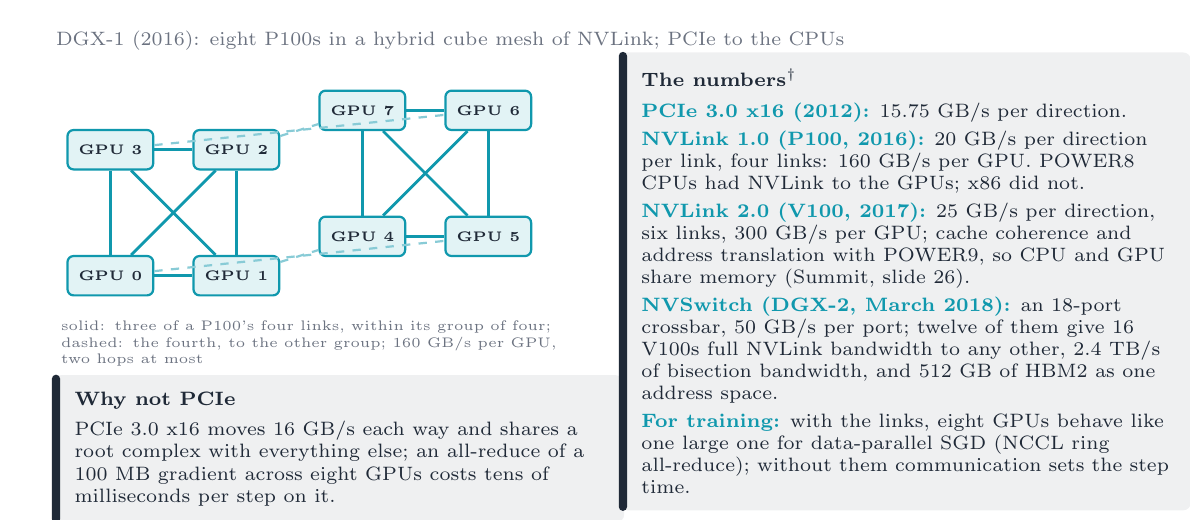
\begin{tikzpicture}
  \useasboundingbox (0,0) rectangle (14.4,5.9);
  \node[lab,anchor=south west] at (0.3,5.55) {DGX-1 (2016): eight P100s in a hybrid cube mesh of NVLink; PCIe to the CPUs};
  \begin{scope}[shift={(0.6,2.45)}]
    \foreach \i/\x/\y in {0/0/0, 1/1.6/0, 2/1.6/1.6, 3/0/1.6, 4/3.2/0.5, 5/4.8/0.5, 6/4.8/2.1, 7/3.2/2.1}{
      \node[comp=vc,minimum width=0.85cm,minimum height=0.5cm,font=\tiny\bfseries,text=ink] (g\i) at (\x+0.45,\y+0.3) {GPU \i};}
    \foreach \a/\b in {0/1,1/2,2/3,3/0,0/2,1/3, 4/5,5/6,6/7,7/4,4/6,5/7}{\draw[vc,line width=1.0pt] (g\a) -- (g\b);}
    \foreach \a/\b in {1/4,2/7,0/5,3/6}{\draw[vc!50,line width=0.8pt,dashed] (g\a) -- (g\b);}
    \node[font=\tiny,text=muted,anchor=north west,text width=6.5cm] at (-0.3,-0.15) {solid: three of a P100's four links, within its group of four; dashed: the fourth, to the other group; 160 GB/s per GPU, two hops at most};
  \end{scope}
  \bgpanels{0.3}{1.5}{6.7cm}{Why not PCIe}{%
    PCIe 3.0 x16 moves 16 GB/s each way and shares a root complex with
    everything else; an all-reduce of a 100 MB gradient across eight
    GPUs costs tens of milliseconds per step on it.}
  \bgpanels{7.5}{5.6}{6.7cm}{The numbers$^\dagger$}{%
    \hl{vc}{PCIe 3.0 x16 (2012):} 15.75 GB/s per direction.\\[2pt]
    \hl{vc}{NVLink 1.0 (P100, 2016):} 20 GB/s per direction per link,
    four links: 160 GB/s per GPU. POWER8 CPUs had NVLink to the GPUs;
    x86 did not.\\[2pt]
    \hl{vc}{NVLink 2.0 (V100, 2017):} 25 GB/s per direction, six links,
    300 GB/s per GPU; cache coherence and address translation with
    POWER9, so CPU and GPU share memory (Summit, slide 26).\\[2pt]
    \hl{vc}{NVSwitch (DGX-2, March 2018):} an 18-port crossbar, 50 GB/s
    per port; twelve of them give 16 V100s full NVLink bandwidth to any
    other, 2.4 TB/s of bisection bandwidth, and 512 GB of HBM2 as one
    address space.\\[2pt]
    \hl{vc}{For training:} with the links, eight GPUs behave like one
    large one for data-parallel SGD (NCCL ring all-reduce); without
    them communication sets the step time.}
\end{tikzpicture}
\end{frame}

% ---------------------------------------------------------------- 26
\begin{frame}{GPUs in supercomputers: Tianhe-1A to Summit}
\framesubtitle{Eight years from the first GPU-accelerated \#1 to a machine where 97\% of the FLOP/s sit on 27{,}648 V100s.}
\centering
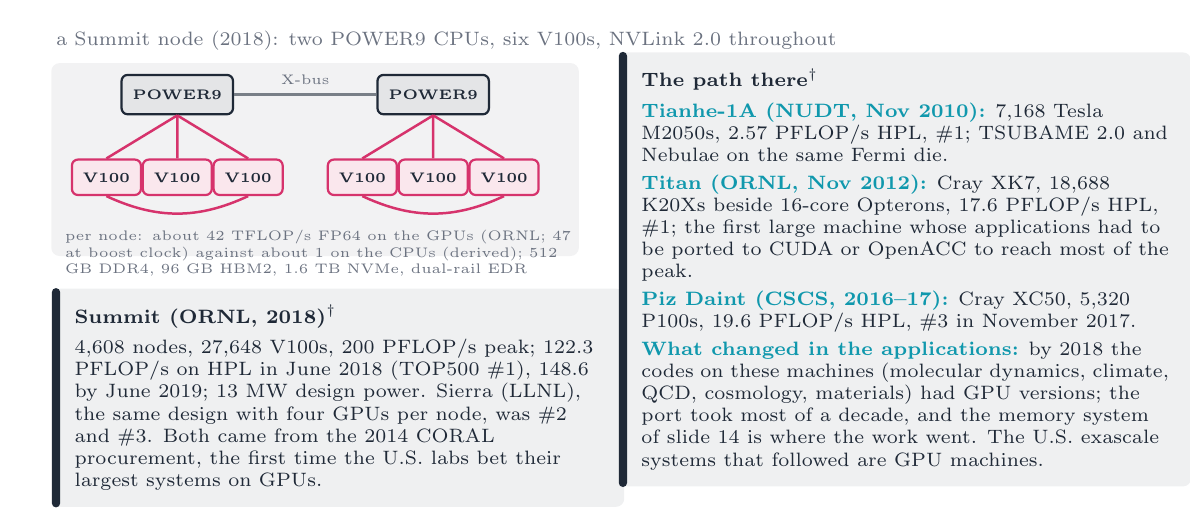
\begin{tikzpicture}
  \useasboundingbox (0,0) rectangle (14.4,5.9);
  \node[lab,anchor=south west] at (0.3,5.55) {a Summit node (2018): two POWER9 CPUs, six V100s, NVLink 2.0 throughout};
  \begin{scope}[shift={(0.3,3.0)}]
    \fill[ink!6,rounded corners=3pt] (0,0) rectangle (6.7,2.45);
    \foreach \s/\x in {0/0.25, 1/3.5}{
      \node[comp=ink,minimum width=1.3cm,minimum height=0.5cm,font=\tiny\bfseries,text=ink] (c\s) at (\x+1.35,2.05) {POWER9};
      \foreach \g in {0,1,2}{\node[comp=outc,minimum width=0.8cm,minimum height=0.45cm,font=\tiny\bfseries,text=ink] (g\s\g) at (\x+0.45+\g*0.9,1.0) {V100};}
      \foreach \g in {0,1,2}{\draw[outc,line width=0.9pt] (c\s.south) -- (g\s\g.north);}
      \draw[outc,line width=0.9pt] (g\s0) -- (g\s1) -- (g\s2); \draw[outc,line width=0.9pt] (g\s0.south) to[bend right=25] (g\s2.south);}
    \draw[ink!60,line width=0.9pt] (c0) -- node[above,font=\tiny,text=muted] {X-bus} (c1);
    \node[font=\tiny,text=muted,anchor=north west,text width=6.5cm] at (0.05,0.45) {per node: about 42 TFLOP/s FP64 on the GPUs (ORNL; 47 at boost clock) against about 1 on the CPUs (derived); 512 GB DDR4, 96 GB HBM2, 1.6 TB NVMe, dual-rail EDR};
  \end{scope}
  \bgpanels{0.3}{2.6}{6.7cm}{Summit (ORNL, 2018)$^\dagger$}{%
    4{,}608 nodes, 27{,}648 V100s, 200 PFLOP/s peak; 122.3 PFLOP/s on
    HPL in June 2018 (TOP500 \#1), 148.6 by June 2019; 13 MW design power. Sierra
    (LLNL), the same design with four GPUs per node, was \#2 and \#3.
    Both came from the 2014 CORAL procurement, the first time the U.S.\
    labs bet their largest systems on GPUs.}
  \bgpanels{7.5}{5.6}{6.7cm}{The path there$^\dagger$}{%
    \hl{vc}{Tianhe-1A (NUDT, Nov 2010):} 7{,}168 Tesla M2050s, 2.57
    PFLOP/s HPL, \#1; TSUBAME 2.0 and Nebulae on the same Fermi die.\\[2pt]
    \hl{vc}{Titan (ORNL, Nov 2012):} Cray XK7, 18{,}688 K20Xs beside
    16-core Opterons, 17.6 PFLOP/s HPL, \#1; the first large machine
    whose applications had to be ported to CUDA or OpenACC to reach
    most of the peak.\\[2pt]
    \hl{vc}{Piz Daint (CSCS, 2016--17):} Cray XC50, 5{,}320 P100s, 19.6
    PFLOP/s HPL, \#3 in November 2017.\\[2pt]
    \hl{vc}{What changed in the applications:} by 2018 the codes on
    these machines (molecular dynamics, climate, QCD, cosmology,
    materials) had GPU versions; the port took most of a decade, and
    the memory system of slide 14 is where the work went. The U.S.\
    exascale systems that followed are GPU machines.}
\end{tikzpicture}
\end{frame}

% ---------------------------------------------------------------- 27
\begin{frame}{The alternatives, and why they lost the decade}
\framesubtitle{AMD's GCN and Vega, Intel's Larrabee and Xeon Phi, and the ``100$\times$'' argument: software and perf/W decided it.}
\centering
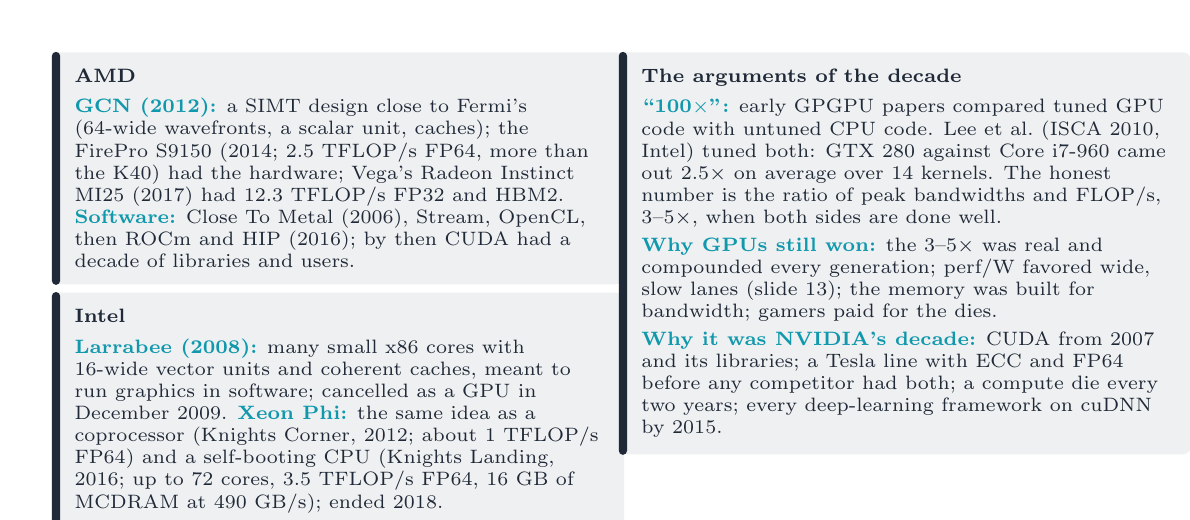
\begin{tikzpicture}
  \useasboundingbox (0,0) rectangle (14.4,5.9);
  \bgpanels{0.3}{5.6}{6.7cm}{AMD}{%
    \hl{vc}{GCN (2012):} a SIMT design close to Fermi's (64-wide
    wavefronts, a scalar unit, caches); the FirePro S9150 (2014; 2.5
    TFLOP/s FP64, more than the K40) had the hardware; Vega's Radeon
    Instinct MI25 (2017) had 12.3 TFLOP/s FP32 and HBM2.
    \hl{vc}{Software:} Close To Metal (2006), Stream, OpenCL, then ROCm
    and HIP (2016); by then CUDA had a decade of libraries and users.}
  \bgpanels{0.3}{2.55}{6.7cm}{Intel}{%
    \hl{vc}{Larrabee (2008):} many small x86 cores with 16-wide vector
    units and coherent caches, meant to run graphics in software;
    cancelled as a GPU in December 2009. \hl{vc}{Xeon Phi:} the same
    idea as a coprocessor (Knights Corner, 2012; about 1 TFLOP/s FP64)
    and a self-booting CPU (Knights Landing, 2016; up to 72 cores, 3.5
    TFLOP/s FP64, 16 GB of MCDRAM at 490 GB/s); ended 2018.}
  \bgpanels{7.5}{5.6}{6.7cm}{The arguments of the decade}{%
    \hl{vc}{``100$\times$'':} early GPGPU papers compared tuned GPU code
    with untuned CPU code. Lee et al.\ (ISCA 2010, Intel) tuned both:
    GTX 280 against Core i7-960 came out 2.5$\times$ on average over 14
    kernels. The honest number is the ratio of peak bandwidths and
    FLOP/s, 3--5$\times$, when both sides are done well.\\[2pt]
    \hl{vc}{Why GPUs still won:} the 3--5$\times$ was real and compounded
    every generation; perf/W favored wide, slow lanes (slide 13); the
    memory was built for bandwidth; gamers paid for the dies.\\[2pt]
    \hl{vc}{Why it was NVIDIA's decade:} CUDA from 2007 and its
    libraries; a Tesla line with ECC and FP64 before any competitor had
    both; a compute die every two years; every deep-learning framework
    on cuDNN by 2015.}
\end{tikzpicture}
\end{frame}

% ---------------------------------------------------------------- 28
\stage{10}
\begin{frame}{What stayed constant for a decade, and what changed}
\framesubtitle{From G80 to Volta the programming model and the SM template held; the counts, memory and datapaths moved.}
\centering
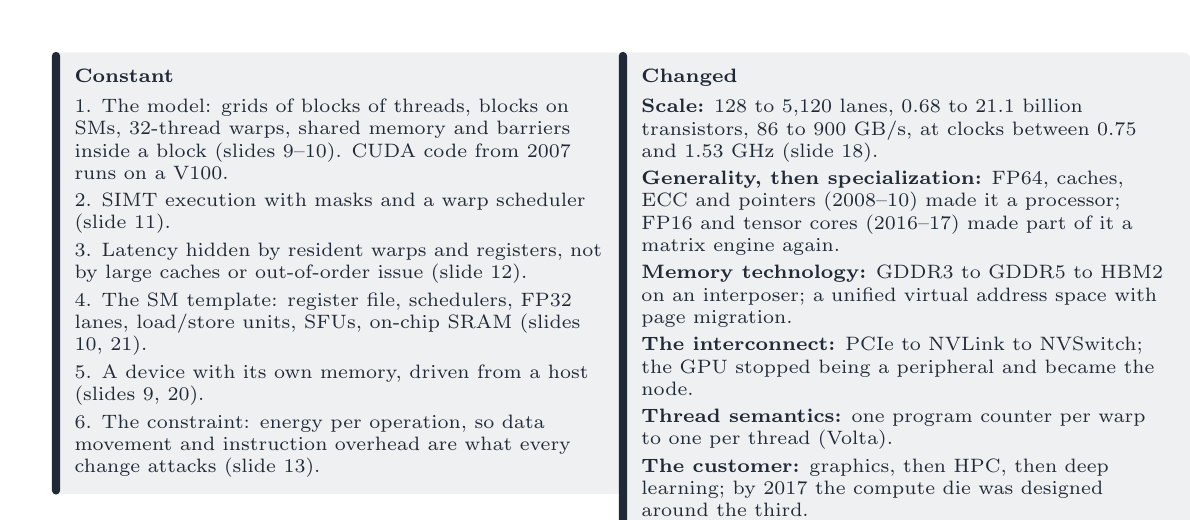
\begin{tikzpicture}
  \useasboundingbox (0,0) rectangle (14.4,5.9);
  \bgpanels{0.3}{5.6}{6.7cm}{Constant}{%
    1. The model: grids of blocks of threads, blocks on SMs, 32-thread
    warps, shared memory and barriers inside a block (slides 9--10).
    CUDA code from 2007 runs on a V100.\\[2pt]
    2. SIMT execution with masks and a warp scheduler (slide 11).\\[2pt]
    3. Latency hidden by resident warps and registers, not by large
    caches or out-of-order issue (slide 12).\\[2pt]
    4. The SM template: register file, schedulers, FP32 lanes,
    load/store units, SFUs, on-chip SRAM (slides 10, 21).\\[2pt]
    5. A device with its own memory, driven from a host (slides 9, 20).\\[2pt]
    6. The constraint: energy per operation, so data movement and
    instruction overhead are what every change attacks (slide 13).}
  \bgpanels{7.5}{5.6}{6.7cm}{Changed}{%
    \hl{ink}{Scale:} 128 to 5{,}120 lanes, 0.68 to 21.1 billion
    transistors, 86 to 900 GB/s, at clocks between 0.75 and 1.53 GHz
    (slide 18).\\[2pt]
    \hl{ink}{Generality, then specialization:} FP64, caches, ECC and
    pointers (2008--10) made it a processor; FP16 and tensor cores
    (2016--17) made part of it a matrix engine again.\\[2pt]
    \hl{ink}{Memory technology:} GDDR3 to GDDR5 to HBM2 on an interposer;
    a unified virtual address space with page migration.\\[2pt]
    \hl{ink}{The interconnect:} PCIe to NVLink to NVSwitch; the GPU
    stopped being a peripheral and became the node.\\[2pt]
    \hl{ink}{Thread semantics:} one program counter per warp to one per
    thread (Volta).\\[2pt]
    \hl{ink}{The customer:} graphics, then HPC, then deep learning; by
    2017 the compute die was designed around the third.}
\end{tikzpicture}
\end{frame}

% ---------------------------------------------------------------- 29
\begin{frame}{In practice: reading a spec sheet, estimating, measuring}
\framesubtitle{First-order performance of a GPU kernel follows from four numbers on the datasheet and one on the kernel.}
\centering
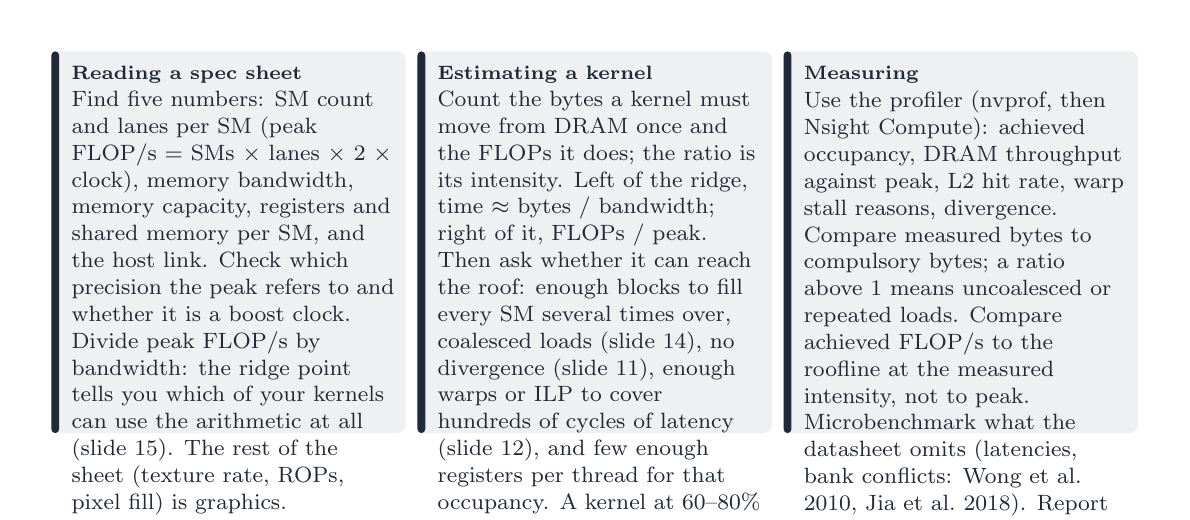
\begin{tikzpicture}
  \useasboundingbox (0,0) rectangle (14.4,5.9);
  \foreach \x/\c/\ttl/\body in {
      0.3/ink/{Reading a spec sheet}/{Find five numbers: SM count and lanes per SM (peak FLOP/s $=$ SMs $\times$ lanes $\times$ 2 $\times$ clock), memory bandwidth, memory capacity, registers and shared memory per SM, and the host link. Check which precision the peak refers to and whether it is a boost clock. Divide peak FLOP/s by bandwidth: the ridge point tells you which of your kernels can use the arithmetic at all (slide 15). The rest of the sheet (texture rate, ROPs, pixel fill) is graphics.},
      4.95/ink/{Estimating a kernel}/{Count the bytes a kernel must move from DRAM once and the FLOPs it does; the ratio is its intensity. Left of the ridge, time $\approx$ bytes $/$ bandwidth; right of it, FLOPs $/$ peak. Then ask whether it can reach the roof: enough blocks to fill every SM several times over, coalesced loads (slide 14), no divergence (slide 11), enough warps or ILP to cover hundreds of cycles of latency (slide 12), and few enough registers per thread for that occupancy. A kernel at 60--80\% of its roofline is done.},
      9.6/ink/{Measuring}/{Use the profiler (nvprof, then Nsight Compute): achieved occupancy, DRAM throughput against peak, L2 hit rate, warp stall reasons, divergence. Compare measured bytes to compulsory bytes; a ratio above 1 means uncoalesced or repeated loads. Compare achieved FLOP/s to the roofline at the measured intensity, not to peak. Microbenchmark what the datasheet omits (latencies, bank conflicts: Wong et al.\ 2010, Jia et al.\ 2018). Report the GPU, clocks, precision and problem size with every number.}}{
    \fill[\c!7,rounded corners=3pt] (\x,0.75) rectangle (\x+4.5,5.6);
    \fill[\c,rounded corners=1.5pt] (\x,0.75) rectangle (\x+0.1,5.6);
    \node[anchor=north west,font=\scriptsize\bfseries,text=\c,inner sep=0,text width=4.1cm] at (\x+0.25,5.42) {\ttl};
    \node[anchor=north west,font=\fontsize{8.0}{9.7}\selectfont,text=ink,inner sep=0,text width=4.1cm,align=flush left] at (\x+0.25,5.1) {\body};}
\end{tikzpicture}
\end{frame}

% ---------------------------------------------------------------- 30
\begin{frame}{Summary: what to take from this lecture}
\framesubtitle{A GPU is a throughput machine: many simple lanes, many threads in flight, a wide memory, and a model that matches.}
\centering
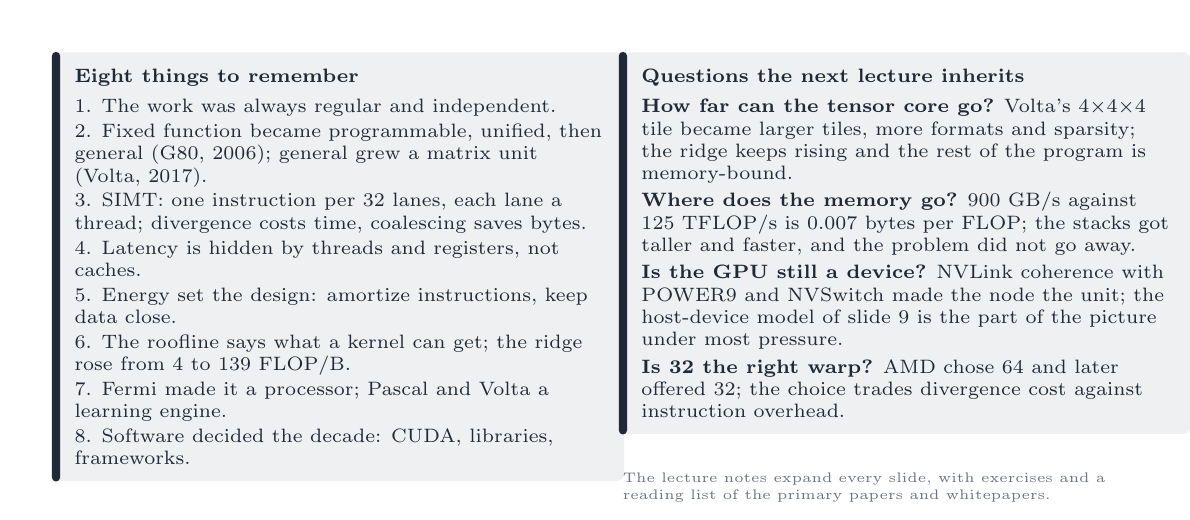
\begin{tikzpicture}
  \useasboundingbox (0,0) rectangle (14.4,5.9);
  \bgpanels{0.3}{5.6}{6.7cm}{Eight things to remember}{%
    1. The work was always regular and independent.\\[1pt]
    2. Fixed function became programmable, unified, then general
    (G80, 2006); general grew a matrix unit (Volta, 2017).\\[1pt]
    3. SIMT: one instruction per 32 lanes, each lane a thread;
    divergence costs time, coalescing saves bytes.\\[1pt]
    4. Latency is hidden by threads and registers, not caches.\\[1pt]
    5. Energy set the design: amortize instructions, keep data close.\\[1pt]
    6. The roofline says what a kernel can get; the ridge rose from 4
    to 139 FLOP/B.\\[1pt]
    7. Fermi made it a processor; Pascal and Volta a learning engine.\\[1pt]
    8. Software decided the decade: CUDA, libraries, frameworks.}
  \bgpanels{7.5}{5.6}{6.7cm}{Questions the next lecture inherits}{%
    \hl{ink}{How far can the tensor core go?} Volta's 4$\times$4$\times$4
    tile became larger tiles, more formats and sparsity; the ridge
    keeps rising and the rest of the program is memory-bound.\\[2pt]
    \hl{ink}{Where does the memory go?} 900 GB/s against 125 TFLOP/s is
    0.007 bytes per FLOP; the stacks got taller and faster, and the
    problem did not go away.\\[2pt]
    \hl{ink}{Is the GPU still a device?} NVLink coherence with POWER9
    and NVSwitch made the node the unit; the host-device model of
    slide 9 is the part of the picture under most pressure.\\[2pt]
    \hl{ink}{Is 32 the right warp?} AMD chose 64 and later offered 32;
    the choice trades divergence cost against instruction overhead.}
  \node[lab,anchor=north west,text width=6.7cm,font=\tiny] at (7.5,0.3) {The lecture notes expand every slide, with exercises and a reading list of the primary papers and whitepapers.};
\end{tikzpicture}
\end{frame}

% ---------------------------------------------------------------- 31
\begin{frame}{Sources}
\framesubtitle{Architecture papers and whitepapers first, then history, then the systems and the debates; $^\dagger$ marks vendor material.}
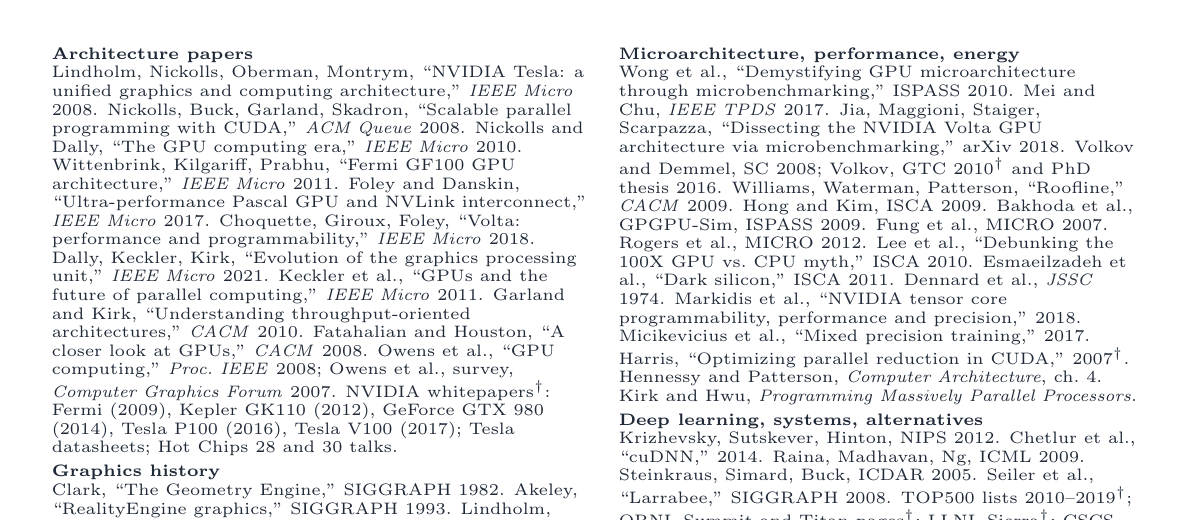
\begin{tikzpicture}
  \useasboundingbox (0,0) rectangle (14.4,5.9);
  \node[anchor=north west,inner sep=0,text width=6.8cm,font=\fontsize{5.6}{6.7}\selectfont,text=ink,align=flush left] at (0.3,5.65) {%
    \textbf{Architecture papers}\\
    Lindholm, Nickolls, Oberman, Montrym, ``NVIDIA Tesla: a unified graphics and computing architecture,'' \emph{IEEE Micro} 2008. Nickolls, Buck, Garland, Skadron, ``Scalable parallel programming with CUDA,'' \emph{ACM Queue} 2008. Nickolls and Dally, ``The GPU computing era,'' \emph{IEEE Micro} 2010. Wittenbrink, Kilgariff, Prabhu, ``Fermi GF100 GPU architecture,'' \emph{IEEE Micro} 2011. Foley and Danskin, ``Ultra-performance Pascal GPU and NVLink interconnect,'' \emph{IEEE Micro} 2017. Choquette, Giroux, Foley, ``Volta: performance and programmability,'' \emph{IEEE Micro} 2018. Dally, Keckler, Kirk, ``Evolution of the graphics processing unit,'' \emph{IEEE Micro} 2021. Keckler et al., ``GPUs and the future of parallel computing,'' \emph{IEEE Micro} 2011. Garland and Kirk, ``Understanding throughput-oriented architectures,'' \emph{CACM} 2010. Fatahalian and Houston, ``A closer look at GPUs,'' \emph{CACM} 2008. Owens et al., ``GPU computing,'' \emph{Proc.\ IEEE} 2008; Owens et al., survey, \emph{Computer Graphics Forum} 2007. NVIDIA whitepapers$^\dagger$: Fermi (2009), Kepler GK110 (2012), GeForce GTX 980 (2014), Tesla P100 (2016), Tesla V100 (2017); Tesla datasheets; Hot Chips 28 and 30 talks.\\[2pt]
    \textbf{Graphics history}\\
    Clark, ``The Geometry Engine,'' SIGGRAPH 1982. Akeley, ``RealityEngine graphics,'' SIGGRAPH 1993. Lindholm, Kilgard, Moreton, ``A user-programmable vertex engine,'' SIGGRAPH 2001. Mark et al., ``Cg,'' SIGGRAPH 2003. Montrym and Moreton, ``The GeForce 6800,'' \emph{IEEE Micro} 2005. Andrews and Baker, ``Xbox 360 system architecture,'' \emph{IEEE Micro} 2006. Blythe, ``The Direct3D 10 system,'' SIGGRAPH 2006. Buck et al., ``Brook for GPUs,'' SIGGRAPH 2004. Peddie, \emph{The History of the GPU} (3 vols., 2022--23).};
  \node[anchor=north west,inner sep=0,text width=6.6cm,font=\fontsize{5.6}{6.7}\selectfont,text=ink,align=flush left] at (7.5,5.65) {%
    \textbf{Microarchitecture, performance, energy}\\
    Wong et al., ``Demystifying GPU microarchitecture through microbenchmarking,'' ISPASS 2010. Mei and Chu, \emph{IEEE TPDS} 2017. Jia, Maggioni, Staiger, Scarpazza, ``Dissecting the NVIDIA Volta GPU architecture via microbenchmarking,'' arXiv 2018. Volkov and Demmel, SC 2008; Volkov, GTC 2010$^\dagger$ and PhD thesis 2016. Williams, Waterman, Patterson, ``Roofline,'' \emph{CACM} 2009. Hong and Kim, ISCA 2009. Bakhoda et al., GPGPU-Sim, ISPASS 2009. Fung et al., MICRO 2007. Rogers et al., MICRO 2012. Lee et al., ``Debunking the 100X GPU vs.\ CPU myth,'' ISCA 2010. Esmaeilzadeh et al., ``Dark silicon,'' ISCA 2011. Dennard et al., \emph{JSSC} 1974. Markidis et al., ``NVIDIA tensor core programmability, performance and precision,'' 2018. Micikevicius et al., ``Mixed precision training,'' 2017. Harris, ``Optimizing parallel reduction in CUDA,'' 2007$^\dagger$. Hennessy and Patterson, \emph{Computer Architecture}, ch.\ 4. Kirk and Hwu, \emph{Programming Massively Parallel Processors}.\\[2pt]
    \textbf{Deep learning, systems, alternatives}\\
    Krizhevsky, Sutskever, Hinton, NIPS 2012. Chetlur et al., ``cuDNN,'' 2014. Raina, Madhavan, Ng, ICML 2009. Steinkraus, Simard, Buck, ICDAR 2005. Seiler et al., ``Larrabee,'' SIGGRAPH 2008. TOP500 lists 2010--2019$^\dagger$; ORNL Summit and Titan pages$^\dagger$; LLNL Sierra$^\dagger$; CSCS Piz Daint$^\dagger$; NVIDIA, AMD, Intel and Khronos press releases$^\dagger$; JEDEC HBM2 (JESD235A) and GDDR5X$^\dagger$. Full list with links in the paper kit.};
\end{tikzpicture}
\end{frame}
\end{document}
